% This file: 			Draft Compiling New Information and Analysis
% Contributors: 		Pietro Biroli, Daniela Del Boca, Linor Kiknadze,
%					Yu Kyung Koh, Sylvi Kuperman, Sidharth Moktan,
%					Chiara Pronzato, Anna Ziff
% Original date: 		10/3/16
% Project: 			Reggio Evaluation

%Style
\documentclass[12pt]{article}
\usepackage[top=1in, bottom=1in, left=1in, right=1in]{geometry}
\parindent 22pt
\usepackage{fancyhdr}

%Packages
\usepackage{adjustbox}
\usepackage{amsmath}
\usepackage{amsfonts}
\usepackage{amssymb}
\usepackage{bm}
\usepackage[table]{xcolor}
\usepackage{tabu}
\usepackage{makecell}
\usepackage{longtable}
\usepackage{multirow}
\usepackage[normalem]{ulem}
\usepackage{etoolbox}
\usepackage{graphicx}
\usepackage{tabularx}
\usepackage{ragged2e}
\usepackage{booktabs}
\usepackage{caption}
\usepackage{fixltx2e}
\usepackage[para, flushleft]{threeparttablex}
\usepackage[capposition=top]{floatrow}
\usepackage{subcaption}
\usepackage{pdfpages}
\usepackage{pdflscape}
\usepackage{natbib}
\usepackage{bibunits}
\definecolor{maroon}{HTML}{990012}
\usepackage[colorlinks=true,linkcolor=maroon,citecolor=maroon,urlcolor=maroon,anchorcolor=maroon]{hyperref}
\usepackage{marvosym}
\usepackage{makeidx}
\usepackage{tikz}
\usetikzlibrary{shapes}
\usepackage{setspace}
\usepackage{enumerate}
\usepackage{rotating}
\usepackage{epstopdf}
\usepackage[titletoc]{appendix}
\usepackage{framed}
\usepackage{comment}
\usepackage{xr}
\usepackage{titlesec}
\usepackage{footnote}
\usepackage{longtable}
\newlength{\tablewidth}
\setlength{\tablewidth}{9.3in}
\setcounter{secnumdepth}{4}

\titleformat{\paragraph}
{\normalfont\normalsize\bfseries}{\theparagraph}{1em}{}
\titlespacing*{\paragraph}
{0pt}{3.25ex plus 1ex minus .2ex}{1.5ex plus .2ex}
\makeatletter
\pretocmd\start@align
{%
  \let\everycr\CT@everycr
  \CT@start
}{}{}
\apptocmd{\endalign}{\CT@end}{}{}
\makeatother
%Watermark
\usepackage[printwatermark]{xwatermark}
\usepackage{lipsum}
\definecolor{lightgray}{RGB}{220,220,220}
%\newwatermark[allpages,color=lightgray,angle=45,scale=3,xpos=0,ypos=0]{Preliminary Draft}

%Further subsection level
\usepackage{titlesec}
\setcounter{secnumdepth}{4}
\titleformat{\paragraph}
{\normalfont\normalsize\bfseries}{\theparagraph}{1em}{}
\titlespacing*{\paragraph}
{0pt}{3.25ex plus 1ex minus .2ex}{1.5ex plus .2ex}

\setcounter{secnumdepth}{5}
\titleformat{\subparagraph}
{\normalfont\normalsize\bfseries}{\thesubparagraph}{1em}{}
\titlespacing*{\subparagraph}
{0pt}{3.25ex plus 1ex minus .2ex}{1.5ex plus .2ex}

%Functions
\DeclareMathOperator{\cov}{Cov}
\DeclareMathOperator{\var}{Var}
\DeclareMathOperator{\plim}{plim}
\DeclareMathOperator*{\argmin}{arg\,min}
\DeclareMathOperator*{\argmax}{arg\,max}

%Math Environments
\newtheorem{theorem}{Theorem}[section]
\newtheorem{claim}[theorem]{Claim}
\newtheorem{assumption}[theorem]{Assumption}
\newtheorem{definition}[theorem]{Definition}
\newtheorem{hypothesis}[theorem]{Hypothesis}
\newtheorem{property}[theorem]{Property}
\newtheorem{example}[theorem]{Example}
\newtheorem{condition}[theorem]{Condition}
\newtheorem{result}[theorem]{Result}
\newenvironment{proof}{\paragraph{Proof:}}{\hfill$\square$}

%Commands
\newcommand\independent{\protect\mathpalette{\protect\independenT}{\perp}}
\def\independenT#1#2{\mathrel{\rlap{$#1#2$}\mkern2mu{#1#2}}}
\newcommand{\overbar}[1]{\mkern 1.5mu\overline{\mkern-1.5mu#1\mkern-1.5mu}\mkern 1.5mu}
\newcommand{\equald}{\ensuremath{\overset{d}{=}}}
\captionsetup[table]{skip=10pt}
%\makeindex


\newcolumntype{L}[1]{>{\raggedright\let\newline\\\arraybackslash\hspace{0pt}}m{#1}}
\newcolumntype{C}[1]{>{\centering\let\newline\\\arraybackslash\hspace{0pt}}m{#1}}
\newcolumntype{R}[1]{>{\raggedleft\let\newline\\\arraybackslash\hspace{0pt}}m{#1}}



%Logo
%\AddToShipoutPictureBG{%
%  \AtPageUpperLeft{\raisebox{-\height}{\includegraphics[width=1.5cm]{uchicago.png}}}
%}

\newcolumntype{L}[1]{>{\raggedright\let\newline\\\arraybackslash\hspace{0pt}}m{#1}}
\newcolumntype{C}[1]{>{\centering\let\newline\\\arraybackslash\hspace{0pt}}m{#1}}
\newcolumntype{R}[1]{>{\raggedleft\let\newline\\\arraybackslash\hspace{0pt}}m{#1}} 

\newcommand{\mr}{\multirow}
\newcommand{\mc}{\multicolumn}

%\newcommand{\comment}[1]{}


\externaldocument{reggioEvaluation_appendix}

\begin{document}

\title{\Large \textbf{Evaluation of the Reggio Approach} \\ Draft}
\author{\normalsize Reggio Team}
\date{\normalsize Original version: October 3, 2016 \\ Current version: \today}
\maketitle

\textbf{[JJH: Many questions -- we are not apologists for Reggio. The \emph{ad hoc} adjustment to matching bothers me. I do not see a good justification and $\Pi$ is estimated. Let's finish. We need to: (1) Put the infant toddler outcomes in main text. We have results. The fact that they are not present in other cities is a huge advantage. (2) Report step down for each column and each table. (3) Identify in each table the group being studied. (4) In the text, we need to summarize main finding of appendix in the text.]}

\tableofcontents

\clearpage
\doublespacing

\section{Introduction}
\label{sec:introduction}

The Reggio Children Approach to Early Childhood Education (the Reggio Approach) is an educational philosophy developed in Reggio Emilia by Loris Malaguzzi in the mid-1900s. This approach has been a source of inspiration for hundreds of early childhood centers that have been created in many countries and in a wide variety of contexts.\footnote{The official \href{http://www.reggiochildren.it/network/?lang=en}{Reggio Children International Network} is present in 33 countries worldwide.} Despite its worldwide recognition, the Reggio Approach has never been formally evaluated, and there is little empirical evidence of its effectiveness. 

The evaluation of the Reggio Approach faces several challenges, given the non-experimental nature of the program and prevalence of other high-quality childcare programs. The northern Italy in the 20th century experienced the development of the early childhood programs that are influenced not only by Malaguzzi but also by other educators. Evidence shows that northern Italy has high-quality, universal early childhood services including the Reggio Approach \citep{OECD_2001_Italy-Country-Note}. Moreover, the take-up rate of childcare in Italy has been increasingly high. The preschool attendence rate of Italian children aged 3-6 years has increased from 50\% in the 1960s to 96\% in the 1990s \citep{Hohnerlein_2015_Development-and-Diffusion}. Therefore, children who are not enrolled in the Reggio Approach preschools have the option of attending other well-established childcare, which makes it difficult to evaluate the effect of the Reggio Approach \textit{per se}. 

This paper presents an evaluation of the Reggio Approach accounting for the challenges mentioned above. Our goal is to compare the Reggio Approach to other programs and understand the similarities and differences between the Reggio Approach and other programs. We have collected data on individuals who have attended each type of early childhood education, as well as those who were informally cared for outside of a center setting. Our sample includes individuals across five age cohorts: three cohorts of adults, one cohort of adolescents, and one cohort of children in their first year of elementary school. The individuals are not only from Reggio Emilia, but also from Padova and Parma, two cities that are similar to Reggio Emilia along several dimensions but have different preschool systems.  

In addition to describing the programs (Section~\ref{sec:eceexperiences}), data (Section~\ref{sec:data}), methods (Section~\ref{sec:methodology}), and results (Section~\ref{sec:result}), we discuss challenges with collecting quality data as well as the historical context that has made construction of a suitable comparison group difficult. We complement discussion of our empirical results with uniquely collated historical records and an original survey administered to officials across the different school systems.

%We find the strongest results comparing adults in their 40s who attended the Reggio Approach with those in Reggio Emilia who did not attend any preschool. These results persist when we make comparisons against those who attended municipal programs in other cities, especially Padova. This is consistent with historical information about the lower availability of alternative preschools at this time and the unavailability of the municipal system in Padova before the age-30 cohorts.

%Although evidence from seminal experiments in early childhood education demonstrates the potential for early childhood education to improve life-cycle outcomes, there are many early childhood interventions implemented with little empirical evidence of their effectiveness.\footnote{For an example of an analysis of the Perry Preschool Program, see \citet{Heckman_Moon_etal_2010_QE}. See \citet{Elango_Hojman_etal_2016_Early-Edu} for an overview of the literature evaluating early childhood education.} The Reggio Approach is one such intervention. Since its inception in 1963 in Reggio Emilia, Italy, the Reggio Approach has been implemented in the municipal schools of Reggio Emilia, as well as replicated internationally.\footnote{The official \href{http://www.reggiochildren.it/network/?lang=en}{Reggio Children International Network} is present in 33 countries worldwide.}

%This paper presents an evaluation the Reggio Approach.\footnote{Although the Reggio Approach includes infant-toddler centers (ages 0-3) and preschools (ages 3-6), we focus our evaluation on the preschools. See Appendix~\ref{sec:asilo_results} for an analysis of the infant-toddler centers.} The Reggio Approach is administrated through the municipal government of Reggio Emilia. Other early childhood education options include state preschools and religious infant-toddler centers and preschools. 

%We have collected data on individuals who have attended each type of early childhood education, as well as those who were informally cared for outside of a center setting. Our sample includes individuals across five age cohorts: three cohorts of adults, one cohort of adolescents, and one cohort of children in their first year of elementary school. The individuals are not only from Reggio Emilia, but also from Padova and Parma, two cities that are similar to Reggio Emilia along several dimensions but have different preschool systems. 

%In addition to describing the programs (Section~\ref{sec:eceexperiences}), data (Section~\ref{sec:data}), methods (Section~\ref{sec:methodology}), and results (Section~\ref{sec:result}), we discuss challenges with collecting quality data as well as the historical context that has made construction of a suitable comparison group difficult. We complement discussion of our empirical results with uniquely collated historical records and an original survey administered to officials across the different school systems.

%We find the strongest results comparing adults in their 40s who attended the Reggio Approach with those in Reggio Emilia who did not attend any preschool. These results persist when we make comparisons against those who attended municipal programs in other cities, especially Padova. This is consistent with historical information about the lower availability of alternative preschools at this time and the unavailability of the municipal system in Padova before the age-30 cohorts.


\section{Childhood Education Experiences in Italy}
\label{sec:ece-italy}
We first document the policies and different types of current early childhood systems in Italy. We then describe the Reggio Approach, which we consider to be the treatment in this evaluation. Because those who did not receive this treatment did not receive a homogenous alternative early childhood education experience, we sought to better understand the history and evolution of various early childhood options apart from what was available in the literature. 

We thus searched municipal archives to document child enrollment and teacher staffing of local schools; we successfully gathered historical materials from the municipal offices of Reggio Emilia and Padova, and from Reggio Children \citep{Padova-Admin-Data_1964-2011,Reggio-Admin-data_1966-2006,Reggio-Annual-Journals_1994-2011}. 

We further conducted a Historical Survey to quantify pedagogical and administrative features of other available childcare experiences available in Reggio Emilia, Parma, and Padova from 1950-2010. We administered the survey to current and retired school administrators and educative coordinators from each system in each city. Survey responses were received that allowed us to document the following programs in each decade from 1950: in Reggio Emilia, municipal and state; in Parma, municipal; and in Padova, municipal, state, and religious. Responses were also received from religious systems in Reggio Emilia and in Parma, however, they did not include historical data prior to 2000. 

We present this survey and its findings to offer a detailed description and comparison of early childhood experiences available to each of the cohorts in this evaluation. See Appendix~\ref{sec:survey} for the list of the administrative and pedagogical components that we inquire about and the full survey.

\subsection{Early Childhood Education in Italy}

Italy's current early childhood policies reflect key state Laws 444 and 1044, passed in 1968 and 1971, mandating the provision and programming of educational childcare by age.\footnote{Prior to 1968, childcare was institutionally provided within the welfare and religious sector for children of working mothers \citep{OECD_2001_Italy-Country-Note,Hohnerlein_2015_Development-and-DiffusionEnrollment}.} The Ministry of Education oversees preschools for children ages 3-6 years; the Ministry of Health is responsible for regulating the provision of infant-toddler childcare for children up to 3 years old \citep{Corsaro_1996_Early-Edu}.\footnote{Current ECE reform efforts seek to unify the system of early childhood education to provide continuity of care from ages 0-6 years \citep{CEHD_2016_Historical-Analysis}.} Accepted literature and administrative records distinguish state and non-state early childhood systems, which include municipal, religious, and secular private programs \citep{Padova-Admin-Data_1964-2011,Reggio-Admin-data_1966-2006,Reggio-Annual-Journals_1994-2011,OECD_2001_Italy-Country-Note,Ribolzi_2013_Italy}. 

Prior to 1968, about 50\% of children aged 3-6 years in Italy were enrolled in childcare provided by non-state institutions \citep{Hohnerlein_2009_Paradox-Public-Preschools}. By 1990, over 96\% of Italian children aged 3-6 years attended preschool, and the state was the main provider \citep{Hohnerlein_2015_Development-and-Diffusion}.\footnote{In contrast, provision of infant-toddler childcare varies considerably across Italy; some municipalities in Northern Italy meet the childcare demand for 30-45\% of families with children under age 3 years, compared to to 2.3\% in the South \citep{Becchi-Ferrari_1990_Pub-Inf-Centres-Italy,Musatti-Picchio_2010_IJEC}.} As the state preschool system expanded, enrollment in religious programs declined from more than 50\% in the 1950s to less than 20\% by 2000. In cities that established high quality municipal programs, fewer children attend state preschool \citep{OECD_2001_Italy-Country-Note}. 

Thus, pursuant to state, regional, and municipal policies, the availability and enrollment in local state and non-state preschool systems for the 5 cohorts in our evaluation varies over time and by city. We summarize this in Table~\ref{tab:itc-pre}. 

\begin{table}[H]
\centering
\caption{Availability of Infant-toddler Centers and Preschools, by City and School Type}\label{tab:itc-pre}
\begin{adjustbox}{width=\textwidth}
\begin{threeparttable}
	\begin{tabular}{l l c c c c c c c c c}
\toprule
\mc{1}{c}{Cohort} & \mc{1}{c}{Years} & \mc{3}{c}{Reggio Emilia} & \mc{3}{c}{Parma} & \mc{3}{c}{Padova} \\
& & Municipal & Catholic & State & Municipal & Catholic & State & Municipal & Catholic & State \\
\midrule
Adults 50s & 1957-1965 & & \checkmark & & & \checkmark & & & \checkmark & \\
Adults 40s & 1972-1976 & \checkmark & \checkmark & & & \checkmark & & & \checkmark & \\
Adults 30s & 1983-1987 & \checkmark & \checkmark & \checkmark & \checkmark & \checkmark & \checkmark & \checkmark & \checkmark & \checkmark \\
Adolescents & 1994-2000 & \checkmark & \checkmark & \checkmark & \checkmark & \checkmark & \checkmark & \checkmark & \checkmark & \checkmark \\
Children & 2009-2014 & \checkmark & \checkmark & \checkmark & \checkmark & \checkmark & \checkmark & \checkmark & \checkmark & \checkmark \\
\bottomrule
\end{tabular}

% Caption:
% Note: This table indicates the types of educational preschool systems (defined as programs with 4 or more sites) available to parents in each city during the years each cohort was eligible for a 3-6 year old program. 
\begin{tablenotes}
Note: This table indicates the main types of educational preschool systems (defined as programs with 4 or more sites) available to parents in each city during the years each cohort was eligible for a 3-6 year old program. 
\end{tablenotes}
\end{threeparttable}
\end{adjustbox}
\end{table}

\subsection{State and Non-State Early Childhood Systems}

Infant-toddler childcare and preschool education are not uniformly regulated, funded, and managed by state and non-state systems. The state does not offer infant-toddler programs. It is currently, however, the largest provider of preschool education for ages 3-6 years. State preschools are only funded where local demand for preschool education is not already met by existing non-state systems \citep{Hohnerlein_2009_Paradox-Public-Preschools}. State preschools charge only for meals and request voluntary contributions from families for extra programming such as field trips \citep{CEHD_2016_Historical-Analysis}. 

Non-state early childhood programs are largely enabled to function autonomously. Access to public funding for non-state schools varies, as does tuition to families. After 2000, state policies were revised to acknowledge non-state schools that complied with eight regulations; `equitable' programs enjoyed increased access to public funds. The distribution of state subsidies for equitable non-state schools is decided by the region \citep{Hohnerlein_2009_Paradox-Public-Preschools,Ribolzi_2013_Italy}. 

The Catholic Church is the oldest non-state early childhood system in Italy, offering both religious training and charitable social services for disadvantaged children since the 19th century \citep{OECD_2001_Italy-Country-Note}. The majority of religious schools enroll children ages 3-6 years; some religious sites offer programming for children beginning at 24 months \citep{Malizia-Cicatelli_2011_BOOK_Catholic-School}. Historically, religious preschools were considered ``schools for the rich'' with tuition purely the family's responsibility \citep{Ribolzi_2013_Italy}. Tuition for religious preschool now depends on family income. 

Municipalities organize and fund community early childhood systems for families with children aged 0-6 years. To comply with key state laws, municipalities must also provide enough infant-toddler ``childcare slots'' to meet local demand \citep{Saraceno_1984_Soc-Probs}. Some municipalities thus contract with private providers to offer a number of infant-toddler and preschool slots according to municipal regulations of eligibility and fees. In general, children of working mothers receive priority enrollment by municipal systems \citep{Saraceno_1984_Soc-Probs}.\footnote{Age of entry into infant-toddler programs varies across municipalities \citep{CEHD_2016_Historical-Analysis}. And while selection criteria are similar across municipalities, the weighting of distinct family characteristics varies \citep{Del-Boca-etal_2016_CESifo-ES}.} Some municipalities provide free preschool while others are offered on a sliding scale. Parental fees for municipal infant-toddler childcare are much higher, covering 21\% of total program costs on average \citep{Musatti-Picchio_2010_IJEC}. 

To summarize, early childhood education in Italy is publicly provided by the state, by the municipality, by religious institutions, and by secular private organizations. Section~\ref{sec:data} describes the selection of our sample into these different school types. 

\subsection{The Reggio Approach}

The Reggio Approach is a form of progressive early childhood education designed by Loris Malaguzzi, an educator influenced by the educational practices and psychological theories of Dewey, Piaget, Erikson, Vygotsky, Bronfenbrenner, Kagan, and Gardner. Malaguzzi, along with Bruno Ciari in Bologna, was one of several left-wing educators within the region of Emilia Romagna who are credited with inciting a `municipal school revolution' in the 1960's. Under the guidance of Malaguzzi, Reggio Emilia opened its first preschool in 1963 for children aged 3-6 years. In 1965, Reggio Emilia passed laws regulating funding for the first infant-toddler center for children aged 3 months to 3 years which later opened in 1971. The Reggio Emilia municipal early childhood system thus preceded Italy's legislative reforms in the 1960s and 1970s that established state-run preschools and mandated the local provision of infant-toddler centers \citep{Cagliari-etal-eds_2016_BOOK_Loris-Malaguzzi}. 

In Reggio Approach preschools, the educative team is assigned specialized roles. Each incoming class of approximately twenty-five 3-year-olds is assigned two full-time co-teachers; at least 1 of the 2 teachers remains with this cohort of homogeneous-aged children for three consecutive years. This extended time provides continuity of care for children and enables strong teacher-family engagement. Each school site is further staffed by a full-time atelierista, an instructor with a background in visual arts. Auxiliary site staff, such as cooks and janitors, are considered members of the educative team and participate in trainings and professional development. A pedagogista---or educative coordinator---with a higher degree in psychology or education is assigned to support professional development on a biweekly basis for the educative staff of approximately 4-5 municipal preschools. 

The Reggio Approach school environment reflects a light-filled, open interior design, furnished with natural materials and a garden. Each site is equipped with an atelier, or dedicated studio laboratory used for creative instructional activities. In-house kitchens are surrounded by glass walls, to include children in the meal process, and is used daily for preparing meals. The Reggio Approach is notable for viewing curriculum as an ongoing, collaborative project without pre-determined learning goals or timelines. There is no institutionally-prescribed content knowledge that educators convey to children for ``school readiness.'' In contrast, teachers and children are viewed as researchers and co-creators of knowledge. For example, educators, children and families collaborate to define a question or topic. Learning is then pursued following a scientific process: theories are shared, tested, and revised through dialogue. Teachers observe children's development, interact with children through questions and dialogue, and provide scaffolding to support learning. Children demonstrate their emerging knowledge through creative learning activities and art, with aid from the atelierista. Teachers document each child's development in a portfolio---a collection of work---which is shared and discussed with children and parents over the year \citep{Rinaldi_2006_ReggioEmilia_BOOK,Giudici-Nicolosi_2014_Reggio-Approach}. 

Reggio Approach preschools and infant-toddler centers are open five full-time days per week from September through June \citep{Giudici-Nicolosi_2014_Reggio-Approach}. Extended day options are available at a majority of Reggio municipal sites throughout the school year, as is educational programming throughout July. Children with disabilities and single parents have been prioritized in admission criteria from the early 1970's \citep{Edwards-etal-eds_1998_Hundred-Languages}. The engagement of families is embedded in Reggio practices, as is the invitation to all community members to participate in school management \citep{CEHD_2016_Historical-Analysis,Cagliari-etal-eds_2016_BOOK_Loris-Malaguzzi}. 


\subsection{Administrative Commonalities}

Results from our survey suggest the following administrative components were shared among municipal systems in each city, state preschools in Padova, and the religious schools of Padova: 

The hours of center-based care is largely shared by the surveyed programs. All systems (except the state preschools in Padova) offered additional hours for working families. Similarly, by the 1990s, all surveyed systems received public funding. Municipal schools in the three cities shared priorities of enrolling economically disadvantaged children, children from a single-parent household, and children with disabilities. 
 
%\subsubsection{Sources of Funding and Costs to Families }
%Until the early 2000s, tuition and fees to families enrolling children in religious preschools in all three cities were relatively more expensive than municipal and state programs. After the 2000s, religious schools acknowledged by the state for meeting quality components were eligible to receive state funding. Public funding across the three school systems is not equitably distributed. 

%Religious schools in Padova did not receive any form of public funding in the 1970s; families were responsible for 100\% of the costs. In the 1980s and 1990s, the municipality of Padova contributed 20\% and 40\% of program costs to religious schools. In the 2000s, families paid 60\% and the remaining 40\% was shared by the state and municipality of Padova. Municipal schools in Padova are free, families pay only for meals. For state schools, families in Padova also make a voluntary contribution, usually to accommodate expenses associated with field trips.\footnote{This information is further supported by an interview with Dr. Emilia Restiglian of University of Padua.}  
 
%Although eligible, the municipality of Reggio Emilia did not receive state funding for its preschool system until the 1990s and 2000s. Ironically, the municipality of Reggio Emilia contributed funds to its state schools each decade since the 1970s. Reggio Emilia also provided training for religious school teachers, beginning in 1994.  

\subsection{Differences Amongst Early Childhood Systems}

Early childhood education systems in Reggio Emilia, Parma, and Padova differ in certain aspects of program administration, environmental features, and pedagogical methods. We describe the alternative early childhood systems below using survey results, administrative municipal records, and published literature.

\subsubsection{Teacher-Child Ratios}

Although in Reggio Emilia, the teacher-child ratio for each classroom has been 2:25 since the 1960s, this number does not reflect the atelierista present at each school site, nor the pedagogista who supervises the educative staff of 4-5 schools. In Padova, the municipal preschool system began to consolidate in 1973, expanding from two to five sites by 1976. Teacher-child ratios for Padova's municipal preschools ranged from 1:12 to 1:24 in 1976. There were three state preschools in Padova by 1976; enrollment was relatively lower and teacher-child ratio approximately 1:15. In this same period, teacher-child ratios at religious schools ranged from 1:34-44.

\subsubsection{State Preschools}

State preschools operate according to legislated policies and \textit{Orientamenti}, or national guidelines defining program standards and general goals for early childhood education. Historically, policies were not consistently enforced throughout Italy, nor were Orientamenti considered binding. They are further revised periodically to reflect current educational practices and political ideology. The first Orientamenti for a system of free state preschools focused on education, development and care were published in 1969 \citep{Corsaro_1996_Early-Edu,Hohnerlein_2015_Development-and-Diffusion}.

The cohorts in our sample thus had differential access to state preschools, and those that attended participated in varying early childhood curricula and administrative practices. While the modern state system was legislated in 1968, historical survey data and administrative records suggest that state preschools did not begin to appear until approximately 1973-1975 in both Reggio Emilia and Padova. The Age 40 cohort, however, had access to 3 or fewer state preschools in each city \citep{Reggio-Admin-data_1966-2006, Reggio-Annual-Journals_1994-2011, Padova-Admin-Data_1964-2011}. This sample is too small to distinguish in our evaluation.\footnote{Administrative from the Municipality of Parma is not available, nor is historical survey data about state preschools in Parma.} 

We thus focus our discussion on the state preschool program as it existed from the late 1970's through the present. By the late 1970's, state policies were reportedly influenced by municipal policies in the region of Emilia Romagna, including Reggio Emilia, Milan, and Pistoia \citep{OECD_2001_Italy-Country-Note}. For example, state preschools a) prioritized enrollment for children with disabilities; b) staffed each classroom with 2 fully trained teachers, and ; c) finally approved the hiring of male teachers \citep{Hohnerlein_2015_Development-and-Diffusion}. In 1980, teacher child-ratio were 2:35; by 1995, teacher-child ratios were reduced to a maximum of 2:25 \citep{Hohnerlein_2009_Paradox-Public-Preschools}. 

In 1991, revised Orientamenti first emphasized social, affective and cognitive development; play, meals, and collaborative skills were defined as the key tasks of early childhood development \citep{Corsaro_1996_Early-Edu}. Further policy revisions in 1997 mandated university degrees and supervised experience for teachers, expanding traditional teacher training from Catholic institutions to secular higher education \citep{Ghedini_2001_Ital-Natl-Policy}. Religious teaching is offered in all state preschools; parents can opt out, however, an alternative educational experiences may not be offered. Teaching methodologies in state preschools include direct instruction as well as play-based learning \citep{CEHD_2016_Historical-Analysis}.

Compared to municipal preschools, teachers in state schools work fewer hours (33/week) than their municipal counterparts who work 36 hours/week. To coordinate legislated maximum working hours and the 8 hour school day, 1 state teacher arrives at 8am, and the other teacher stays until all parents arrive for pick up time. Children in state preschools thus spend more time in a classroom staffed by only 1 teacher than those in municipal schools. Teachers in state preschools further have less weekly time set aside for professional training, documentation, and engagement of parents.

\subsubsection{Parma Municipal Schools}

Detailed documentation of the Parma municipal early childhood system is scarce. Conversation with the authors of \citet{Edwards-etal-eds_1998_Hundred-Languages} suggests that the pedagogical approach of Parma's municipal system is similar to that of Reggio Emilia.\footnote{Kuperman, Interview with Carolyn Pope Edwards, 2016.} One relevant difference for this evaluation is that Parma's municipal system consolidated and expanded around 1975, about a decade after Reggio Emilia. 

As of 2001, Parma provided 16 infant-toddler centers throughout the municipality. Pedagogical coordinators perform both administrative and professional development roles. Assigned to a specific set of infant-toddler centers, these coordinators meet twice each month with all teachers collectively for shared reflection, on-site supervision, and to promote relationships with the families. The city director meets biweekly with all pedagogical coordinators for overall planning. University professors or administrators from other municipalities provide professional development in the form of continuing education \citep{Terzi-Cantarelli_2001_Parma}. Parma's infant-toddler centers are intentionally designed in the context of an apartment. \citet{Terzi-Cantarelli_2001_Parma} report mixed-age classes that include 18 total children from 13 months to 3 years in a single section, led by two teachers (9:1 child-teacher ratio). To accommodate parents, infant-toddler centers open at 7:30pm and offer three pick-up times: 2 p.m. (short-day), 3:30 p.m. (normal-day), or 5 p.m. (extended-day). Classrooms can be organized by single-age groups (e.g., 5-12 months, 12-24 months, and 24-36 months) or by mixed-age groups (e.g.,12-36 months) \citep{Majorano-etal_2009_CC-in-P}.

\subsubsection{Padova Municipal Schools}

Padova is located in the relatively more religious and politically diverse region of Veneto. Compared to Reggio Emilia and Parma, its municipal early childhood education system is smaller, offering 10 preschool centers. In contrast, Padova has a larger number of religious preschool centers. In 1989, the region of Veneto reported a total provision of childcare slots for 3.9\% of its infant-toddler population. In contrast, the region of Emilia Romagna reported a provision of infant-toddler childcare for 15.6\% of its population. The practice of professional development trainings for early childhood staff in Veneto first began in 1986 \citep{Becchi-Ferrari_1990_Pub-Inf-Centres-Italy}.

In Padova, the municipal preschool system began to consolidate in 1973, expanding from two to five sites by 1976. Teacher-child ratios for Padova's municipal preschools ranged from 1:12 to 1:24 in 1976 \citep{Padova-Admin-Data_1964-2011,CEHD_2016_Historical-Analysis}.

\subsubsection{Catholic Schools}

The Catholic Church offers religious early childhood education. The Catholic Church is greatly concerned with equity and parity of state funding for its non-state schools. Unlike municipal systems, the majority of costs for private religious preschool are subsidized by tuition paid by enrolled families. Private schools historically were considered options only for affluent families that could afford the tuition expense \citep{Hohnerlein_2009_Paradox-Public-Preschools}.\footnote{Prior to 2000, state funding for private schools reflected a 1947 constitutional clause that non-state schools could operate ``without financial burdens on the state.'' Today, depending on their income and the particular municipality's subsidy program, families enrolled in religious programs are eligible for subsidized tuition \citep{Hohnerlein_2009_Paradox-Public-Preschools}. In 2005, however, funding for state and private schools differed greatly. While equitable religious preschools could receive state funds, funding for religious primary schools (ages 6-11 years) was at 15.5\% the rate of public primary schools. Private secondary schools (ages 11-18 years) received no state funding \citep{Becchi-Ferrari_1990_Pub-Inf-Centres-Italy}.}

By 1976; teacher-child ratios at Padova's religious schools ranged from 1:34-44. Prior to revised state policies in 1997-2000, Catholic preschools were taught by nuns, teacher training was not publicly mandated, and teacher-child ratios were relatively low. Coincidentally, religious programs began to hire trained, secular teachers who implemented varied curricula. In the north, traditional instruction began to incorporate some active-child learning, and some sites began to provide entry to children at age 24 months.

Until the early 2000s, tuition and fees to families enrolling children in religious preschools in all three cities were relatively more expensive than municipal and state programs. Religious schools in Padova did not receive any form of public funding in the 1970s; families were responsible for 100\% of the costs. In the 1980s and 1990s, the municipality of Padova contributed 20\% and 40\% of program costs to religious schools. In the 2000s, families paid 60\% and the remaining 40\% was shared by the state and municipality of Padova. After the 2000s, religious schools acknowledged by the state for meeting quality components were eligible to receive state funding.\footnote{This information comes from a variety of sources: \citet{Reggio-Admin-data_1966-2006, Reggio-Annual-Journals_1994-2011, Padova-Admin-Data_1964-2011} and results from the survey \citep{CEHD_2016_Historical-Analysis}},





%\subsubsection{Infant-Toddler Programs} eligible age of entry for infant-toddler programs varies from 3 months in Reggio Emilia to 9 months in Padova


\section{Research Design}
\label{sec:data}
\subsection{The Selection of Cities}

Our dataset contains cohorts of individuals raised in Parma and Padova, in addition to Reggio Emilia. Parma and Padova are similar to Reggio Emilia in terms of geography, population, and socio-economic structure, but they do not have the Reggio Approach available.\footnote{Other Italian cities were taken into consideration, notably Brescia, Livorno, Modena, Perugia, Piacenza, Prato, and Ravenna. Parma and Padova were the two cities that best fulfilled our comparability and sample requirements.} 

All three cities are in Northern Italy with Parma and Reggio Emilia being in the same province and Padova being in the neighboring one. In addition to geographic proximity, they have similar populations as seen in Figure~\ref{fig:population}. Although the population in Padova is larger than in Parma and Reggio Emilia, the trends are similar across time. These similar trends can also be seen in the migration rates between the three cities (Figure~\ref{fig:emigr-immigr}). Although emigration rate is highest in Padova and net migration rate is highest in Reggio Emilia for most of the years, general trends in emigration and immigration in similar in all cities. Trends in foreign migration are almost identical in three cities. 

The similarities between the cities are also seen in economic terms. Reggio Emilia has an average per-capita income of 25,226 euros, Parma of 28,437, and Padova of 29,915 in 2011 \citep{Comuni-Italiani_2017_Redditi-Ipref-per-Regione-2011}. Other economic information, such as unemployment, is similar across the cities as well. We present more information on the three cities in Appendix~\ref{sec:data-app}. 

\begin{figure}[H]
      \begin{center}
        \begin{subfigure}[t]{0.49\textwidth}
          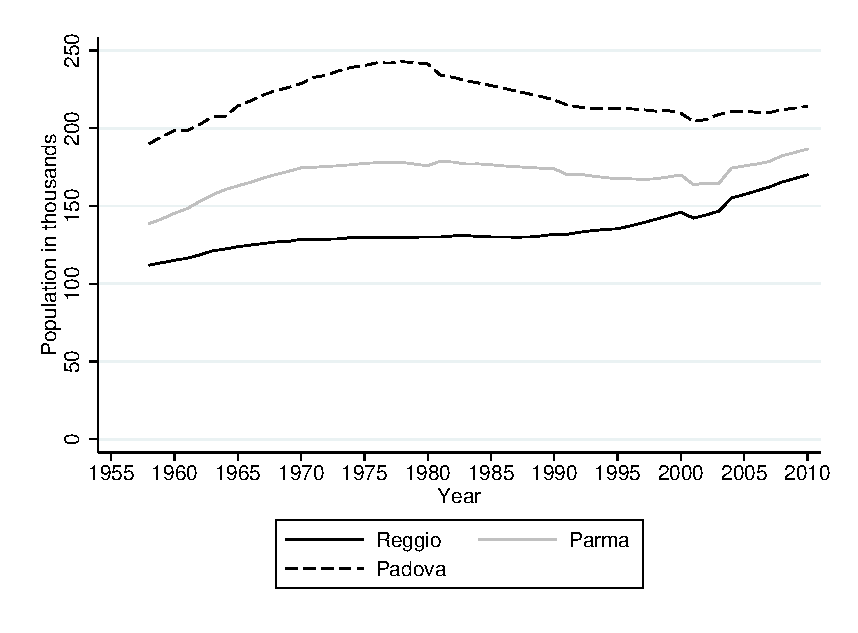
\includegraphics[width=\textwidth]{../../output/image/population.eps}
\caption{Population}
        \end{subfigure}
        \begin{subfigure}[t]{0.49\textwidth}
          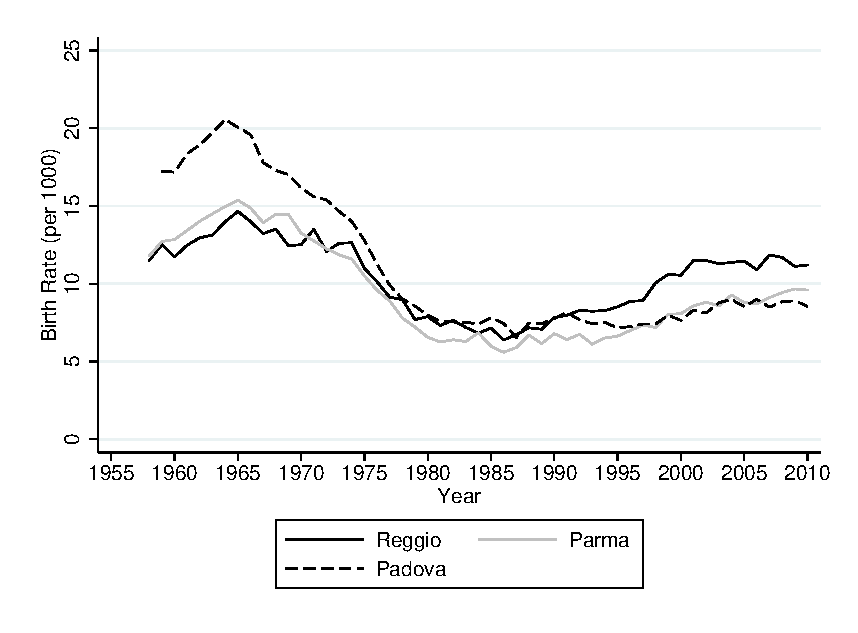
\includegraphics[width=\textwidth]{../../output/image/birth_rate.eps}
 \caption{Birth Rate}
        \end{subfigure}
        \begin{subfigure}[t]{0.49\textwidth}
          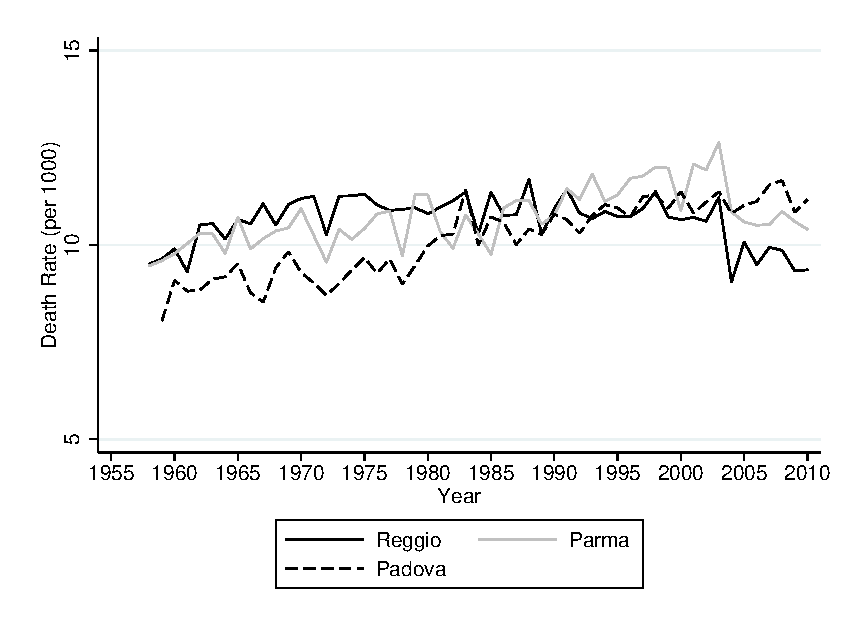
\includegraphics[width=\textwidth]{../../output/image/death_rate.eps}
        \caption{Death Rate}
        \end{subfigure}
        \begin{subfigure}[t]{0.49\textwidth}
          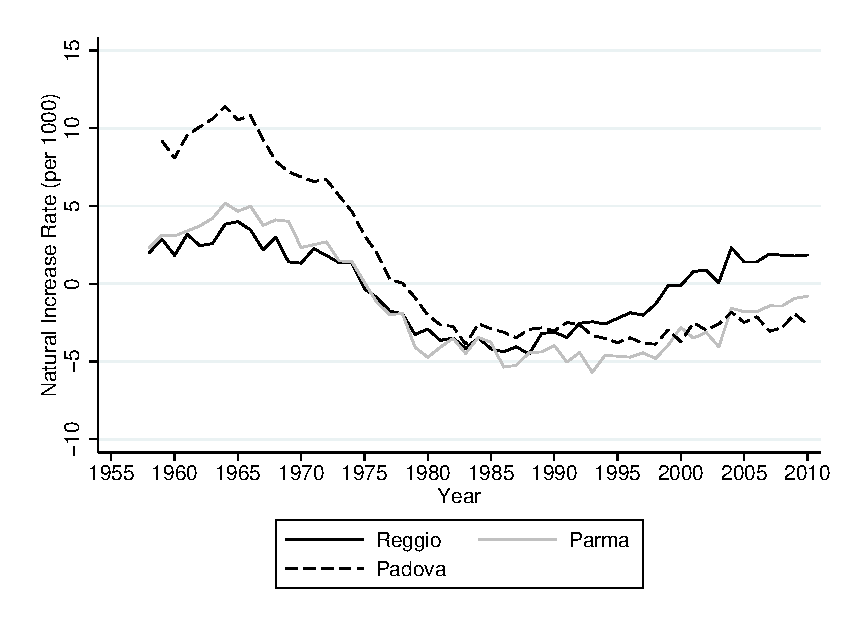
\includegraphics[width=\textwidth]{../../output/image/naturalinc_rate.eps}
            \caption{Natural Rate}
        \end{subfigure}
      \caption{Population Statistics}  \label{fig:population}
      \end{center}
      \raggedright Note: See Appendix~\ref{sec:data-app} for more information on these data and the sources.
    \end{figure}

\begin{figure}[H]
      \begin{center}
        \begin{subfigure}[t]{0.49\textwidth}
          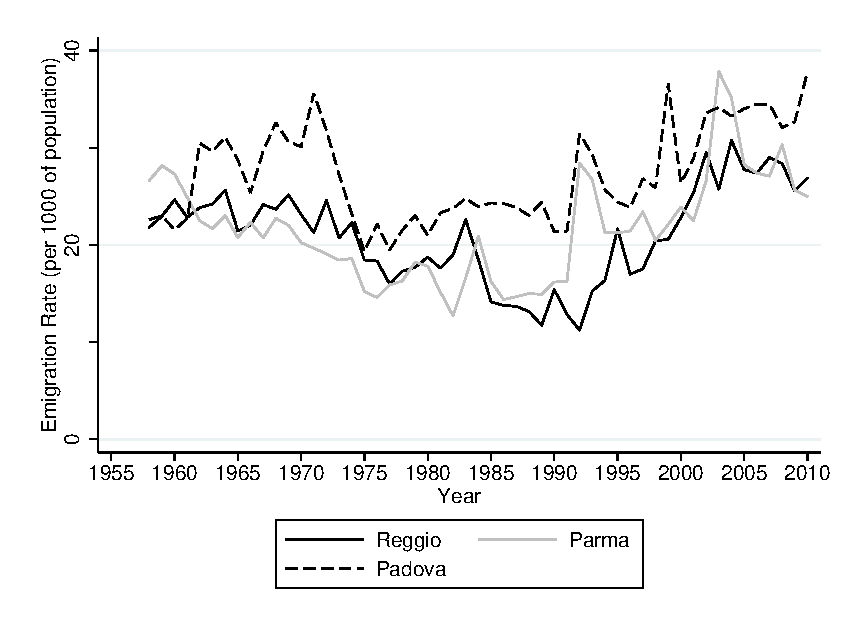
\includegraphics[width=\textwidth]{../../output/image/emigration.eps}
            \caption{Emigration}
        \end{subfigure}
      \begin{subfigure}[t]{0.49\textwidth}
        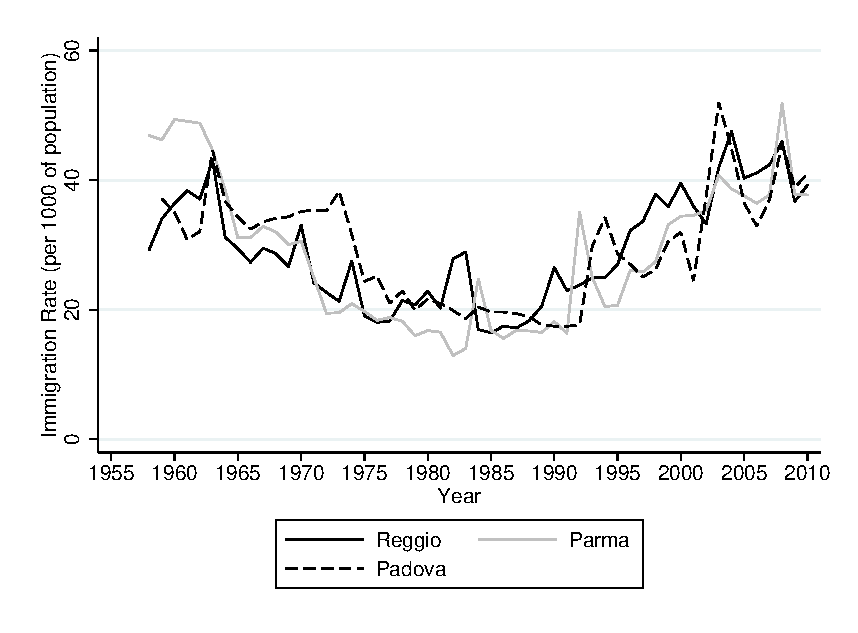
\includegraphics[width=\textwidth]{../../output/image/immigration.eps}
        \caption{Immigration}
      \end{subfigure}
	 \begin{subfigure}[t]{0.49\textwidth}
          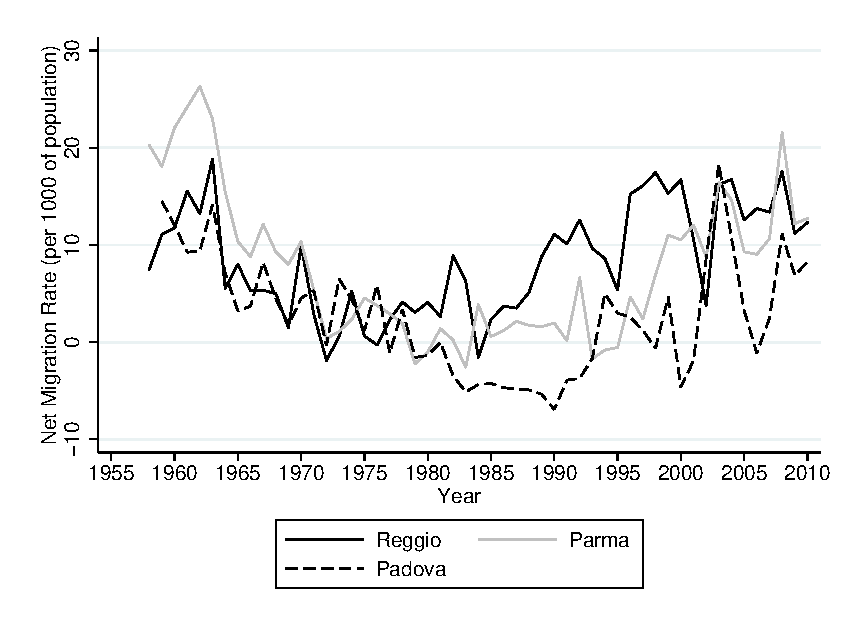
\includegraphics[width=\textwidth]{../../output/image/netmigration.eps}
\caption{Net Migration}
        \end{subfigure}
        \begin{subfigure}[t]{0.49\textwidth}
          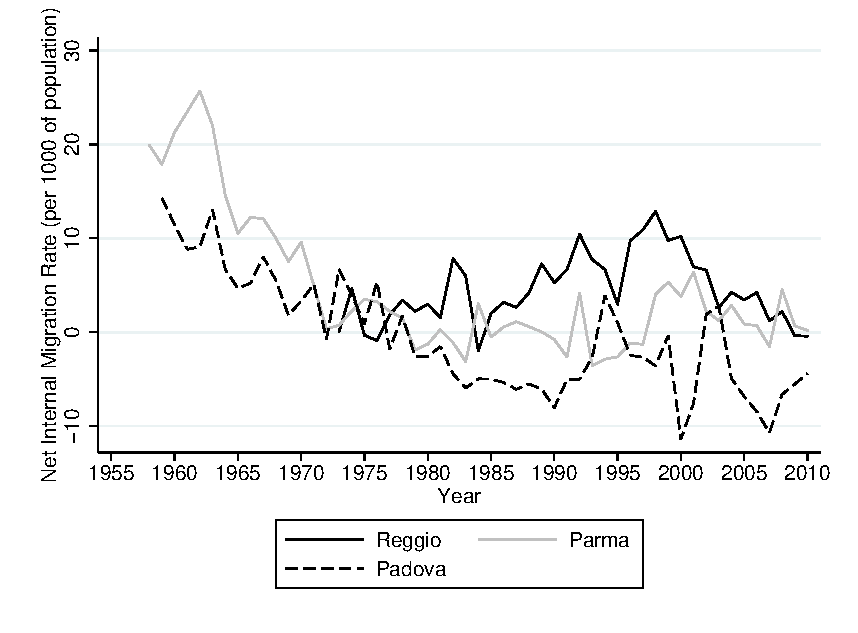
\includegraphics[width=\textwidth]{../../output/image/netinternalmig.eps}
 \caption{Net Internal Migration}
        \end{subfigure}
        \begin{subfigure}[ht]{0.48\textwidth}
          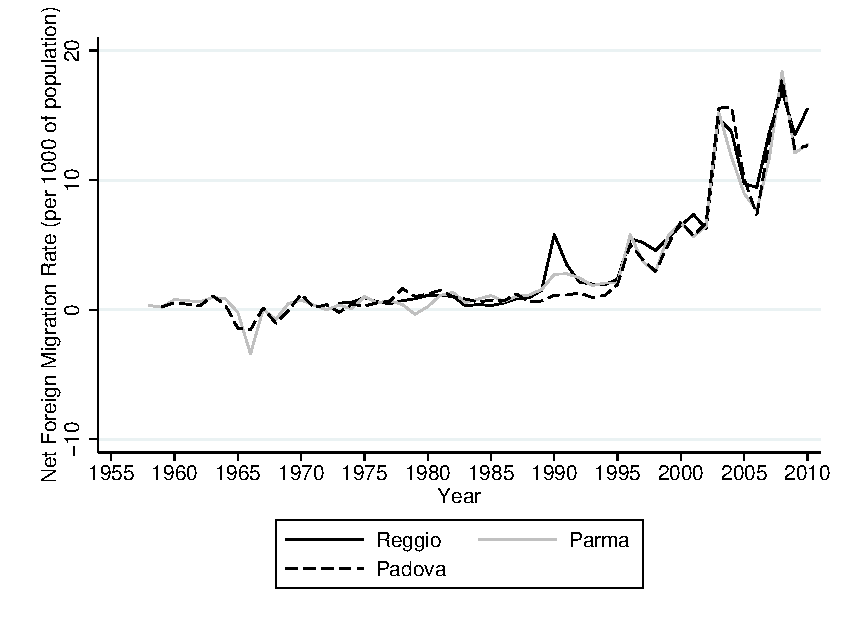
\includegraphics[width=\textwidth]{../../output/image/netforeignmig.eps}
        \caption{Net Foreign Migration}
        \end{subfigure}
      \caption{Migration Statistics}  \label{fig:emigr-immigr}
      \end{center}
         \raggedright  Note: See Appendix~\ref{sec:data-app} for more information on these data and the sources.
    \end{figure}
   
   \textbf{[JJH: Can we test for equality across cities?][We moved these figures from the appendix to help show the similarity between the cities. We also started a table below summarizing these variables aggregating across years. We test for equality here. Is this what you had in mind?]}
    We summarize the main population statistics in Table~\ref{tab:pop-summary-stat} in which we present the mean and standard deviations of the population, birth rate, death rate, and net migration across years.
    

    \begin{table}[H]
    \centering
    \caption{Summarizing Population Statistics Across Cities} \label{tab:pop-summary-stat}
    \begin{threeparttable}
	
	\begin{tabular}{l c c c}
\toprule
&	Reggio Emilia & Parma & Padova \\
\midrule
Population	& 134,459.6 &   \textbf{170,335} &  \textbf{219,161.2}   \\
			& (13,413.67) & (10,104.85)& (13,474.66)   \\
Birth rate & 		10.38 &9.36  & 	11.08 \\
	(per 1,000)	&		(2.33) & (3.02) & (4.55) \\
Death rate &  10.62 &  10.74 & \textbf{10.13} \\
	(per 1,000)	& (0.63) & (0.74) & (095) \\
Net migration & 8.40 &  7.38 & \textbf{2.68} \\
	(per 1,000)		& (5.63) & (7.36) & (5.96) \\
\bottomrule
\end{tabular}


\begin{tablenotes}
\item \footnotesize Note: This table summarizes the average of population statistics across available years by city. We use a $t$-test to compare the means and bold those that are significant at least at the 0.05 level. Standard deviations are reported in parentheses. See Appendix~\ref{sec:data-app} for more information on these data and the sources.
\end{tablenotes}
\end{threeparttable}
\end{table}
	
    
The sample is a subset of the individuals in Reggio Emilia, Parma, and Padova who were born in the year ranges of the five cohorts.  These individuals were collected from the population registries in each of the cities. The sample was then restricted to those individuals living in the same city in which they were raised. All cohorts except the youngest one comprised only individuals who are Italian citizens. In contrast, the youngest cohort includes an oversampling of immigrant children.\footnote{In the adult cohorts there was no immigrant who was born in the any of the three cities and still lived there. In the adolescent cohort, the number was immigrant born was extremely small.} The sample from Reggio Emilia, across all cohorts, includes an oversampling of those who attended municipal schools, as this is the treatment group.

Of the reference sample, 7,109 individuals were randomly selected. Of these, 4,019 completed interviews, resulting in a response rate of 56.5\%. Table~\ref{tab:sample-city-cohort} provides an overview of the birth years for the different cohorts and the counts of the full sample.
\begin{table}[H]
\centering
\begin{threeparttable}
	\caption{Description of the Full Sample by Cohort and City}\label{tab:sample-city-cohort}
	\begin{tabular}{l c c c c c c}
\toprule
Cohort & Birth year(s) & Age at interview & \mc{4}{c}{Count} \\
\cmidrule{4-7}
 & 		&						& Reggio Emilia & Parma & Padova & \textbf{Total} \\
\midrule
\textbf{Children} &  &  &  & &  &  \\ 
\quad Italians & 2006 & 6 & 311 & 291& 278 & 880 \\
\quad Migrants & 2006 & 6 & 110 & 58 & 113 & 281 \\
\textbf{Adolescents} & 1994 & 19 & 300 & 254 & 282 & 836 \\
\textbf{Adults 30s} & 1980-1981 & 32 & 280 & 251 & 251 & 782 \\
\textbf{Adults 40s} & 1969-1970 & 43 & 285 & 254 & 252 & 791 \\
\textbf{Adults 50s} & 1954-1959 & 54-60 & 200 & 103 & 146 & 449 \\
\midrule
\textbf{Total}	& 				& & 1,486 & 1,211 & 1,322 & 4,019 \\
\bottomrule
\end{tabular}
\begin{tablenotes}
\footnotesize
Note: This table presents the number of individuals in the full sample. The age at interview is an approximation given there is some variation in the interview date and birth year within each cohort.
\end{tablenotes}
\end{threeparttable}
\end{table}

Table~\ref{tab:sample} provides a detailed tabulation of the sample by city, cohort, and school type. It is shown that the number of people who do not attend any preschool significantly decreases over time. Whereas the majority of people from age-50 cohort did not attend any preschool, there are only few people among children, migrants, and adolescents who did not attend any preschool. Table \ref{tab:sample} also shows that the proportion of people attending municipal preschools is higher in Reggio than in other cities. 


\begin{table}[H]
\centering
\scalebox{0.58}{
\begin{threeparttable}
	\caption{Tabulation by Cohort, City, and School Type}\label{tab:sample}
	\begin{tabular}{l*{22}{c}}
\toprule
            &\mc{7}{c}{Reggio Emilia: 1,486}   &     \mc{7}{c}{ Parma: 1,211}       &      \mc{7}{c}{Padova: 1,322}      \\
           \cmidrule(lr){2-8} \cmidrule(lr){9-15} \cmidrule(lr){16-22} 
	&	None	&	Muni	&	State	&	Reli	&	Priv	&	Affi	&	Other	&	None	&	Muni	&	State	&	Reli	&	Priv	&	Affi	&	Other	&	None	&	Muni	&	State	&	Reli	&	Private	&	Affi	&	Other	\\ \midrule
Children	&	2	&	158	&	45	&	91	&	5	&	9	&	0	&	6	&	39	&	43	&	77	&	9	&	115	&	0	&	2	&	58	&	45	&	141	&	12	&	19	&	0	\\
Migrants	&	4	&	48	&	37	&	14	&	1	&	4	&	0	&	4	&	8	&	10	&	3	&	6	&	27	&	0	&	5	&	36	&	47	&	23	&	1	&	0	&	0	\\
Adolescents	&	7	&	151	&	22	&	97	&	6	&	14	&	0	&	4	&	43	&	43	&	82	&	6	&	73	&	0	&	1	&	85	&	47	&	132	&	6	&	7	&	0	\\
Adult 30s	&	57	&	146	&	31	&	40	&	1	&	4	&	0	&	44	&	60	&	53	&	50	&	5	&	36	&	0	&	47	&	27	&	27	&	140	&	1	&	7	&	0	\\
Adult 40s	&	80	&	119	&	17	&	52	&	5	&	1	&	8	&	116	&	0	&	0	&	55	&	1	&	33	&	45	&	75	&	0	&	0	&	126	&	0	&	10	&	38	\\
Adult 50s	&	147	&	0	&	0	&	28	&	2	&	0	&	20	&	72	&	0	&	0	&	11	&	0	&	10	&	9	&	57	&	0	&	0	&	72	&	2	&	6	&	3	\\

\bottomrule
\end{tabular}


\begin{tablenotes}
Note: This table shows the sample size by city, cohort, and school type. We separate migrants and children for clarity in this table even though they are in the same birth cohort (year of birth: 2006). None: no preschool; Muni.: municipal preschool;  State: state preschool; Relig.: religious preschool; Priv.: private preschool. Affi: municipal-affiliated preschool; Other: uncategorized preschool.
\end{tablenotes}
\end{threeparttable}
}
\end{table}

The structure of the cohorts allows us to study the effects of the Reggio Approach at different points throughout the life cycle. The children in the youngest cohort were interviewed when they entered primary school, the adolescent cohort when they ended compulsory schooling, and the adult cohorts capture different points of adulthood to measure key outcomes such as engagement in the labor market, health, and family decisions. This cohort structure also allows us to evaluate the Reggio Approach compared to the alternative early childhood experiences over time.

Separate questionnaires were administered to the children, adolescents, and adults. as well as to the caregivers of the children and adolescents. The questionnaires include items about early childhood experiences, family structure, education, interaction with non-Italians (or with Italians in the case of the migrant children), and measures of cognitive and social-emotional skills. The questionnaires for adults additionally included items about occupation, income, health, and life satisfaction. 

%Table \ref{table:summaryStat_baseline} presents summary statistics for baseline variables by cohort and city. As mentioned above, certain baseline variables are missing for the adult cohorts due to differences in questionnaires administered to adults and children. The table illustrates differences and similarities in parental, caregiver and family characteristics across cities as well as over time.

%\begin{landscape}
%\singlespace
\setlength{\tabcolsep}{2pt}
\begin{center}
\scriptsize{
\begin{longtable}{L{6cm} c c c p{.5cm} c c c p{.5cm} c c c p{.5cm} c c c p{.5cm} c c c}
\hline\multicolumn{20}{L{24cm}}{\textbf{Note:} Means are reported for each variable by cohort and city. Standard Deviations are reported in italics below each mean estimate. A . denotes that the variable is not defined for a specific cohort.}
\endfoot
\caption{Summary statistics for baseline variables by cohort and city} \label{table:summaryStat_baseline} \\
\hline
& \multicolumn{3}{c}{\textbf{Children}} & & \multicolumn{3}{c}{\textbf{Adolescents}} & & \multicolumn{3}{c}{\textbf{Adults 30}} & & \multicolumn{3}{c}{\textbf{Adults 40}} & & \multicolumn{3}{c}{\textbf{Adults 50}}\\
& \scriptsize{Reggio} & \scriptsize{Parma}& \scriptsize{Padova} & & \scriptsize{Reggio} & \scriptsize{Parma}& \scriptsize{Padova} & & \scriptsize{Reggio} & \scriptsize{Parma}& \scriptsize{Padova} & & \scriptsize{Reggio} & \scriptsize{Parma}& \scriptsize{Padova} & & \scriptsize{Reggio} & \scriptsize{Parma}& \scriptsize{Padova}\\
\hline \\[.2em] \endhead
 \quad Male & 0.54 &      0.56 &      0.52 & &      0.43 &      0.44 &      0.48 & &      0.60 &      0.53 &      0.55 & &      0.54 &      0.49 &      0.48 & &      0.47 &      0.38 &      0.46 \\*
 \quad & $\mathit{     0.50}$ & $\mathit{     0.50}$ & $\mathit{     0.50}$ & & $\mathit{     0.50}$ & $\mathit{     0.50}$ & $\mathit{     0.50}$ & & $\mathit{     0.49}$ & $\mathit{     0.50}$ & $\mathit{     0.50}$ & & $\mathit{     0.50}$ & $\mathit{     0.50}$ & $\mathit{     0.50}$ & & $\mathit{     0.50}$ & $\mathit{     0.49}$ & $\mathit{     0.50}$ \\[.2em]
 \quad Low birthweight & 0.08 &      0.07 &      0.05 & &      0.05 &      0.06 &      0.05 & &         . &         . &         . & &         . &         . &         . & &         . &         . &         . \\*
 \quad & $\mathit{     0.27}$ & $\mathit{     0.25}$ & $\mathit{     0.21}$ & & $\mathit{     0.23}$ & $\mathit{     0.24}$ & $\mathit{     0.21}$ & & $\mathit{        .}$ & $\mathit{        .}$ & $\mathit{        .}$ & & $\mathit{        .}$ & $\mathit{        .}$ & $\mathit{        .}$ & & $\mathit{        .}$ & $\mathit{        .}$ & $\mathit{        .}$ \\[.2em]
 \quad Premature birth & 0.10 &      0.08 &      0.07 & &      0.06 &      0.10 &      0.07 & &         . &         . &         . & &         . &         . &         . & &         . &         . &         . \\*
 \quad & $\mathit{     0.30}$ & $\mathit{     0.26}$ & $\mathit{     0.25}$ & & $\mathit{     0.24}$ & $\mathit{     0.30}$ & $\mathit{     0.25}$ & & $\mathit{        .}$ & $\mathit{        .}$ & $\mathit{        .}$ & & $\mathit{        .}$ & $\mathit{        .}$ & $\mathit{        .}$ & & $\mathit{        .}$ & $\mathit{        .}$ & $\mathit{        .}$ \\[.2em]
 \quad CAPI & 0.55 &      0.43 &      0.47 & &      0.43 &      0.55 &      0.49 & &      0.57 &      0.40 &      0.35 & &      0.63 &      0.34 &      0.35 & &      0.45 &      0.35 &      0.28 \\*
 \quad & $\mathit{     0.50}$ & $\mathit{     0.50}$ & $\mathit{     0.50}$ & & $\mathit{     0.50}$ & $\mathit{     0.50}$ & $\mathit{     0.50}$ & & $\mathit{     0.50}$ & $\mathit{     0.49}$ & $\mathit{     0.48}$ & & $\mathit{     0.48}$ & $\mathit{     0.48}$ & $\mathit{     0.48}$ & & $\mathit{     0.50}$ & $\mathit{     0.48}$ & $\mathit{     0.45}$ \\[.2em]
 \quad Born to teenaged mother & 0.00 &      0.01 &      0.01 & &      0.01 &      0.02 &      0.00 & &      1.00 &      1.00 &      1.00 & &      1.00 &      1.00 &      1.00 & &      1.00 &      1.00 &      1.00 \\*
 \quad & $\mathit{     0.00}$ & $\mathit{     0.08}$ & $\mathit{     0.08}$ & & $\mathit{     0.11}$ & $\mathit{     0.12}$ & $\mathit{     0.00}$ & & $\mathit{     0.00}$ & $\mathit{     0.00}$ & $\mathit{     0.00}$ & & $\mathit{     0.00}$ & $\mathit{     0.00}$ & $\mathit{     0.00}$ & & $\mathit{     0.00}$ & $\mathit{     0.00}$ & $\mathit{     0.00}$ \\[.2em]
 \quad Mom born in province & 0.51 &      0.60 &      0.69 & &      0.68 &      0.68 &      0.78 & &      0.84 &      0.70 &      0.71 & &      0.80 &      0.74 &      0.63 & &      0.78 &      0.80 &      0.76 \\*
 \quad & $\mathit{     0.50}$ & $\mathit{     0.49}$ & $\mathit{     0.46}$ & & $\mathit{     0.47}$ & $\mathit{     0.47}$ & $\mathit{     0.41}$ & & $\mathit{     0.36}$ & $\mathit{     0.46}$ & $\mathit{     0.46}$ & & $\mathit{     0.40}$ & $\mathit{     0.44}$ & $\mathit{     0.48}$ & & $\mathit{     0.42}$ & $\mathit{     0.40}$ & $\mathit{     0.43}$ \\[.2em]
 \quad Mom Max Edu: Low & 0.17 &      0.07 &      0.10 & &      0.16 &      0.11 &      0.14 & &      0.00 &      0.00 &      0.00 & &      0.02 &      0.00 &      0.00 & &      0.01 &      0.04 &      0.01 \\*
 \quad & $\mathit{     0.38}$ & $\mathit{     0.25}$ & $\mathit{     0.30}$ & & $\mathit{     0.36}$ & $\mathit{     0.31}$ & $\mathit{     0.35}$ & & $\mathit{     0.06}$ & $\mathit{     0.00}$ & $\mathit{     0.00}$ & & $\mathit{     0.13}$ & $\mathit{     0.00}$ & $\mathit{     0.06}$ & & $\mathit{     0.10}$ & $\mathit{     0.19}$ & $\mathit{     0.12}$ \\[.2em]
 \quad Mom Max Edu: Middle School & 0.08 &      0.05 &      0.09 & &      0.09 &      0.10 &      0.11 & &      0.03 &      0.07 &      0.10 & &      0.19 &      0.24 &      0.23 & &      0.41 &      0.55 &      0.64 \\*
 \quad & $\mathit{     0.27}$ & $\mathit{     0.23}$ & $\mathit{     0.29}$ & & $\mathit{     0.29}$ & $\mathit{     0.30}$ & $\mathit{     0.31}$ & & $\mathit{     0.18}$ & $\mathit{     0.25}$ & $\mathit{     0.30}$ & & $\mathit{     0.39}$ & $\mathit{     0.43}$ & $\mathit{     0.42}$ & & $\mathit{     0.49}$ & $\mathit{     0.50}$ & $\mathit{     0.48}$ \\[.2em]
 \quad Mom Max Edu: High School & 0.45 &      0.41 &      0.45 & &      0.48 &      0.44 &      0.43 & &      0.42 &      0.30 &      0.35 & &      0.47 &      0.35 &      0.35 & &      0.36 &      0.26 &      0.18 \\*
 \quad & $\mathit{     0.50}$ & $\mathit{     0.49}$ & $\mathit{     0.50}$ & & $\mathit{     0.50}$ & $\mathit{     0.50}$ & $\mathit{     0.50}$ & & $\mathit{     0.49}$ & $\mathit{     0.46}$ & $\mathit{     0.48}$ & & $\mathit{     0.50}$ & $\mathit{     0.48}$ & $\mathit{     0.48}$ & & $\mathit{     0.48}$ & $\mathit{     0.44}$ & $\mathit{     0.39}$ \\[.2em]
 \quad Mom Max Edu: University & 0.28 &      0.46 &      0.36 & &      0.25 &      0.33 &      0.29 & &      0.55 &      0.63 &      0.54 & &      0.31 &      0.41 &      0.41 & &      0.22 &      0.15 &      0.15 \\*
 \quad & $\mathit{     0.45}$ & $\mathit{     0.50}$ & $\mathit{     0.48}$ & & $\mathit{     0.43}$ & $\mathit{     0.47}$ & $\mathit{     0.46}$ & & $\mathit{     0.50}$ & $\mathit{     0.48}$ & $\mathit{     0.50}$ & & $\mathit{     0.46}$ & $\mathit{     0.49}$ & $\mathit{     0.49}$ & & $\mathit{     0.42}$ & $\mathit{     0.35}$ & $\mathit{     0.36}$ \\[.2em]
 \quad Born to teenaged father & 0.00 &      0.00 &      0.01 & &      0.00 &      0.01 &      0.00 & &      1.00 &      1.00 &      1.00 & &      1.00 &      1.00 &      1.00 & &      1.00 &      1.00 &      1.00 \\*
 \quad & $\mathit{     0.00}$ & $\mathit{     0.06}$ & $\mathit{     0.08}$ & & $\mathit{     0.00}$ & $\mathit{     0.09}$ & $\mathit{     0.06}$ & & $\mathit{     0.00}$ & $\mathit{     0.00}$ & $\mathit{     0.00}$ & & $\mathit{     0.00}$ & $\mathit{     0.00}$ & $\mathit{     0.00}$ & & $\mathit{     0.00}$ & $\mathit{     0.00}$ & $\mathit{     0.00}$ \\[.2em]
 \quad Father born in province & 0.52 &      0.59 &      0.64 & &      0.58 &      0.61 &      0.73 & &      0.87 &      0.79 &      0.76 & &      0.78 &      0.85 &      0.73 & &      0.84 &      0.65 &      0.82 \\*
 \quad & $\mathit{     0.50}$ & $\mathit{     0.49}$ & $\mathit{     0.48}$ & & $\mathit{     0.49}$ & $\mathit{     0.49}$ & $\mathit{     0.44}$ & & $\mathit{     0.34}$ & $\mathit{     0.41}$ & $\mathit{     0.43}$ & & $\mathit{     0.42}$ & $\mathit{     0.36}$ & $\mathit{     0.44}$ & & $\mathit{     0.37}$ & $\mathit{     0.48}$ & $\mathit{     0.38}$ \\[.2em]
 \quad Dad Max Edu: Low & 0.23 &      0.12 &      0.09 & &      0.19 &      0.16 &      0.14 & &         . &         . &         . & &      0.02 &      0.00 &      0.00 & &      0.01 &      0.04 &      0.02 \\*
 \quad & $\mathit{     0.42}$ & $\mathit{     0.33}$ & $\mathit{     0.29}$ & & $\mathit{     0.40}$ & $\mathit{     0.37}$ & $\mathit{     0.35}$ & & $\mathit{        .}$ & $\mathit{        .}$ & $\mathit{        .}$ & & $\mathit{     0.14}$ & $\mathit{     0.06}$ & $\mathit{     0.06}$ & & $\mathit{     0.07}$ & $\mathit{     0.19}$ & $\mathit{     0.14}$ \\[.2em]
 \quad Dad Max Edu: Middle School & 0.08 &      0.10 &      0.09 & &      0.09 &      0.07 &      0.10 & &      0.03 &      0.08 &      0.10 & &      0.19 &      0.22 &      0.14 & &      0.35 &      0.55 &      0.52 \\*
 \quad & $\mathit{     0.27}$ & $\mathit{     0.30}$ & $\mathit{     0.28}$ & & $\mathit{     0.28}$ & $\mathit{     0.26}$ & $\mathit{     0.30}$ & & $\mathit{     0.17}$ & $\mathit{     0.27}$ & $\mathit{     0.30}$ & & $\mathit{     0.39}$ & $\mathit{     0.41}$ & $\mathit{     0.35}$ & & $\mathit{     0.48}$ & $\mathit{     0.50}$ & $\mathit{     0.50}$ \\[.2em]
 \quad Dad Max Edu: High School & 0.35 &      0.36 &      0.42 & &      0.40 &      0.36 &      0.39 & &      0.37 &      0.32 &      0.32 & &      0.45 &      0.33 &      0.27 & &      0.36 &      0.19 &      0.17 \\*
 \quad & $\mathit{     0.48}$ & $\mathit{     0.48}$ & $\mathit{     0.49}$ & & $\mathit{     0.49}$ & $\mathit{     0.48}$ & $\mathit{     0.49}$ & & $\mathit{     0.48}$ & $\mathit{     0.47}$ & $\mathit{     0.47}$ & & $\mathit{     0.50}$ & $\mathit{     0.47}$ & $\mathit{     0.44}$ & & $\mathit{     0.48}$ & $\mathit{     0.40}$ & $\mathit{     0.38}$ \\[.2em]
 \quad Dad Max Edu: University & 0.24 &      0.35 &      0.30 & &      0.19 &      0.26 &      0.28 & &      0.60 &      0.60 &      0.57 & &      0.33 &      0.45 &      0.58 & &      0.27 &      0.20 &      0.27 \\*
 \quad & $\mathit{     0.43}$ & $\mathit{     0.48}$ & $\mathit{     0.46}$ & & $\mathit{     0.39}$ & $\mathit{     0.44}$ & $\mathit{     0.45}$ & & $\mathit{     0.49}$ & $\mathit{     0.49}$ & $\mathit{     0.50}$ & & $\mathit{     0.47}$ & $\mathit{     0.50}$ & $\mathit{     0.49}$ & & $\mathit{     0.45}$ & $\mathit{     0.40}$ & $\mathit{     0.45}$ \\[.2em]
 \quad Has 1 sibling & 0.52 &      0.46 &      0.50 & &      0.52 &      0.46 &      0.55 & &      0.36 &      0.33 &      0.45 & &      0.36 &      0.38 &      0.35 & &      0.28 &      0.26 &      0.39 \\*
 \quad & $\mathit{     0.50}$ & $\mathit{     0.50}$ & $\mathit{     0.50}$ & & $\mathit{     0.50}$ & $\mathit{     0.50}$ & $\mathit{     0.50}$ & & $\mathit{     0.48}$ & $\mathit{     0.47}$ & $\mathit{     0.50}$ & & $\mathit{     0.48}$ & $\mathit{     0.49}$ & $\mathit{     0.48}$ & & $\mathit{     0.45}$ & $\mathit{     0.44}$ & $\mathit{     0.49}$ \\[.2em]
 \quad Has 2 siblings & 0.14 &      0.21 &      0.17 & &      0.18 &      0.20 &      0.15 & &      0.24 &      0.33 &      0.25 & &      0.27 &      0.33 &      0.35 & &      0.30 &      0.27 &      0.22 \\*
 \quad & $\mathit{     0.35}$ & $\mathit{     0.41}$ & $\mathit{     0.37}$ & & $\mathit{     0.38}$ & $\mathit{     0.40}$ & $\mathit{     0.36}$ & & $\mathit{     0.43}$ & $\mathit{     0.47}$ & $\mathit{     0.43}$ & & $\mathit{     0.44}$ & $\mathit{     0.47}$ & $\mathit{     0.48}$ & & $\mathit{     0.46}$ & $\mathit{     0.45}$ & $\mathit{     0.42}$ \\[.2em]
 \quad Has more than 2 siblings & 0.06 &      0.04 &      0.05 & &      0.09 &      0.06 &      0.02 & &      0.13 &      0.20 &      0.17 & &      0.20 &      0.19 &      0.26 & &      0.34 &      0.39 &      0.35 \\*
 \quad & $\mathit{     0.23}$ & $\mathit{     0.19}$ & $\mathit{     0.21}$ & & $\mathit{     0.29}$ & $\mathit{     0.24}$ & $\mathit{     0.16}$ & & $\mathit{     0.33}$ & $\mathit{     0.40}$ & $\mathit{     0.37}$ & & $\mathit{     0.40}$ & $\mathit{     0.39}$ & $\mathit{     0.44}$ & & $\mathit{     0.48}$ & $\mathit{     0.49}$ & $\mathit{     0.48}$ \\[.2em]
 \quad Caregiver was Catholic & 0.77 &      0.83 &      0.79 & &      0.75 &      0.86 &      0.73 & &         . &         . &         . & &         . &         . &         . & &         . &         . &         . \\*
 \quad & $\mathit{     0.42}$ & $\mathit{     0.37}$ & $\mathit{     0.41}$ & & $\mathit{     0.43}$ & $\mathit{     0.35}$ & $\mathit{     0.44}$ & & $\mathit{        .}$ & $\mathit{        .}$ & $\mathit{        .}$ & & $\mathit{        .}$ & $\mathit{        .}$ & $\mathit{        .}$ & & $\mathit{        .}$ & $\mathit{        .}$ & $\mathit{        .}$ \\[.2em]
 \quad Caregiver was faithful and Catholic & 0.47 &      0.52 &      0.51 & &      0.45 &      0.54 &      0.45 & &         . &         . &         . & &         . &         . &         . & &         . &         . &         . \\*
 \quad & $\mathit{     0.50}$ & $\mathit{     0.50}$ & $\mathit{     0.50}$ & & $\mathit{     0.50}$ & $\mathit{     0.50}$ & $\mathit{     0.50}$ & & $\mathit{        .}$ & $\mathit{        .}$ & $\mathit{        .}$ & & $\mathit{        .}$ & $\mathit{        .}$ & $\mathit{        .}$ & & $\mathit{        .}$ & $\mathit{        .}$ & $\mathit{        .}$ \\[.2em]
 \quad Caregiver owned house & 0.58 &      0.71 &      0.66 & &      0.84 &      0.81 &      0.77 & &         . &         . &         . & &         . &         . &         . & &         . &         . &         . \\*
 \quad & $\mathit{     0.49}$ & $\mathit{     0.46}$ & $\mathit{     0.48}$ & & $\mathit{     0.37}$ & $\mathit{     0.39}$ & $\mathit{     0.42}$ & & $\mathit{        .}$ & $\mathit{        .}$ & $\mathit{        .}$ & & $\mathit{        .}$ & $\mathit{        .}$ & $\mathit{        .}$ & & $\mathit{        .}$ & $\mathit{        .}$ & $\mathit{        .}$ \\[.2em]
 \quad Caregiver was a migrant & 0.07 &      0.02 &      0.02 & &      0.01 &      0.02 &      0.00 & &         . &         . &         . & &         . &         . &         . & &         . &         . &         . \\*
 \quad & $\mathit{     0.26}$ & $\mathit{     0.14}$ & $\mathit{     0.15}$ & & $\mathit{     0.11}$ & $\mathit{     0.12}$ & $\mathit{     0.00}$ & & $\mathit{        .}$ & $\mathit{        .}$ & $\mathit{        .}$ & & $\mathit{        .}$ & $\mathit{        .}$ & $\mathit{        .}$ & & $\mathit{        .}$ & $\mathit{        .}$ & $\mathit{        .}$ \\[.2em]
 \quad Caregiver Income: 5,000 euros or less & 0.01 &      0.02 &      0.03 & &      0.00 &      0.02 &      0.04 & &         . &         . &         . & &         . &         . &         . & &         . &         . &         . \\*
 \quad & $\mathit{     0.11}$ & $\mathit{     0.15}$ & $\mathit{     0.18}$ & & $\mathit{     0.06}$ & $\mathit{     0.15}$ & $\mathit{     0.19}$ & & $\mathit{        .}$ & $\mathit{        .}$ & $\mathit{        .}$ & & $\mathit{        .}$ & $\mathit{        .}$ & $\mathit{        .}$ & & $\mathit{        .}$ & $\mathit{        .}$ & $\mathit{        .}$ \\[.2em]
 \quad Caregiver Income: 5,001-10,000 euros & 0.01 &      0.02 &      0.01 & &      0.01 &      0.01 &      0.01 & &         . &         . &         . & &         . &         . &         . & &         . &         . &         . \\*
 \quad & $\mathit{     0.11}$ & $\mathit{     0.13}$ & $\mathit{     0.12}$ & & $\mathit{     0.10}$ & $\mathit{     0.09}$ & $\mathit{     0.08}$ & & $\mathit{        .}$ & $\mathit{        .}$ & $\mathit{        .}$ & & $\mathit{        .}$ & $\mathit{        .}$ & $\mathit{        .}$ & & $\mathit{        .}$ & $\mathit{        .}$ & $\mathit{        .}$ \\[.2em]
 \quad Caregiver Income: 10,001-25,000 euros & 0.17 &      0.19 &      0.15 & &      0.18 &      0.18 &      0.10 & &         . &         . &         . & &         . &         . &         . & &         . &         . &         . \\*
 \quad & $\mathit{     0.38}$ & $\mathit{     0.39}$ & $\mathit{     0.36}$ & & $\mathit{     0.39}$ & $\mathit{     0.38}$ & $\mathit{     0.30}$ & & $\mathit{        .}$ & $\mathit{        .}$ & $\mathit{        .}$ & & $\mathit{        .}$ & $\mathit{        .}$ & $\mathit{        .}$ & & $\mathit{        .}$ & $\mathit{        .}$ & $\mathit{        .}$ \\[.2em]
 \quad Caregiver Income: 25,001-50,000 euros & 0.32 &      0.41 &      0.32 & &      0.32 &      0.29 &      0.24 & &         . &         . &         . & &         . &         . &         . & &         . &         . &         . \\*
 \quad & $\mathit{     0.47}$ & $\mathit{     0.49}$ & $\mathit{     0.47}$ & & $\mathit{     0.47}$ & $\mathit{     0.46}$ & $\mathit{     0.43}$ & & $\mathit{        .}$ & $\mathit{        .}$ & $\mathit{        .}$ & & $\mathit{        .}$ & $\mathit{        .}$ & $\mathit{        .}$ & & $\mathit{        .}$ & $\mathit{        .}$ & $\mathit{        .}$ \\[.2em]
 \quad Caregiver Income: 50,001-100,000 euros & 0.19 &      0.19 &      0.13 & &      0.24 &      0.24 &      0.11 & &         . &         . &         . & &         . &         . &         . & &         . &         . &         . \\*
 \quad & $\mathit{     0.40}$ & $\mathit{     0.39}$ & $\mathit{     0.34}$ & & $\mathit{     0.43}$ & $\mathit{     0.43}$ & $\mathit{     0.31}$ & & $\mathit{        .}$ & $\mathit{        .}$ & $\mathit{        .}$ & & $\mathit{        .}$ & $\mathit{        .}$ & $\mathit{        .}$ & & $\mathit{        .}$ & $\mathit{        .}$ & $\mathit{        .}$ \\[.2em]
 \quad Caregiver Income: 100,001-250,000 euros & 0.02 &      0.02 &      0.03 & &      0.04 &      0.03 &      0.02 & &         . &         . &         . & &         . &         . &         . & &         . &         . &         . \\*
 \quad & $\mathit{     0.15}$ & $\mathit{     0.14}$ & $\mathit{     0.17}$ & & $\mathit{     0.20}$ & $\mathit{     0.17}$ & $\mathit{     0.16}$ & & $\mathit{        .}$ & $\mathit{        .}$ & $\mathit{        .}$ & & $\mathit{        .}$ & $\mathit{        .}$ & $\mathit{        .}$ & & $\mathit{        .}$ & $\mathit{        .}$ & $\mathit{        .}$ \\[.2em]
 \quad Caregiver Income: > 250,000 euros & . &         . &         . & &      0.00 &      0.00 &      0.00 & &         . &         . &         . & &         . &         . &         . & &         . &         . &         . \\*
 \quad & $\mathit{        .}$ & $\mathit{        .}$ & $\mathit{        .}$ & & $\mathit{     0.06}$ & $\mathit{     0.00}$ & $\mathit{     0.00}$ & & $\mathit{        .}$ & $\mathit{        .}$ & $\mathit{        .}$ & & $\mathit{        .}$ & $\mathit{        .}$ & $\mathit{        .}$ & & $\mathit{        .}$ & $\mathit{        .}$ & $\mathit{        .}$ \\[.2em]
 \quad Caregiver was religious & 0.85 &      0.87 &      0.80 & &      0.77 &      0.87 &      0.74 & &      0.50 &      0.73 &      0.72 & &      0.50 &      0.75 &      0.75 & &      0.64 &      0.71 &      0.77 \\*
 \quad & $\mathit{     0.36}$ & $\mathit{     0.34}$ & $\mathit{     0.40}$ & & $\mathit{     0.42}$ & $\mathit{     0.34}$ & $\mathit{     0.44}$ & & $\mathit{     0.50}$ & $\mathit{     0.45}$ & $\mathit{     0.45}$ & & $\mathit{     0.50}$ & $\mathit{     0.43}$ & $\mathit{     0.44}$ & & $\mathit{     0.48}$ & $\mathit{     0.46}$ & $\mathit{     0.42}$ \\[.2em]
 ~\\[-.5em]
\hline
\end{longtable}
}
\end{center}

%\end{landscape}

\subsection{Characteristics of Reggio Emilia, Parma, and Padova}

Parma and Padova are similar to Reggio Emilia along several characteristics, but have different early childhood education offerings.\footnote{See Appendix Section~\ref{sec:eceexperiences} for a discussion of the differences in early childhood education in the three cities.} All three cities are in Northern Italy; Reggio Emilia and Parma are in the same region of Emilia Romagna, Padova is in the adjacent region of Veneto. 
%Tables~\ref{table:demo-employ} and~\ref{table:demo-other} describe the cities along demographic characteristics. Reggio Emilia and Parma, in addition to being geographically close are socially and economically similar.

The three cities are similar in employment for different industries, proportion of individuals renting property, and marital status. In 2011, Padova had more individuals with post-secondary degrees compared with Reggio Emilia and Parma. Starting in 1991, the aging index has been higher in Parma than in Reggio Emilia. Starting in 2001, Padova's aging index overtook that of both Reggio Emilia and Parma. A higher aging index indicates there are more individuals over 59 years of age per one hundred individuals under 15 years of age, i.e., an older population with low birth rates. Appendix \ref{app:characteristics-cities} has more detailed information about demographic characteristics of Reggio, Parma, and Padova. 

%\begin{landscape}
%\begin{table}[ht!]
%\begin{center}
%\scriptsize{
%	\caption{Proportion of Individuals in Different Employment and Industry Categories} \label{table:demo-employ}
%	
\begin{tabular}{L{6.5cm} *{3}{*{5}{c} c}}
\hline \\[-7pt]
& \multicolumn{5}{c}{\textbf{Reggio Emilia}} & & \multicolumn{5}{c}{\textbf{Parma}} & & \multicolumn{5}{c}{\textbf{Padova}} \\[3pt]
& \textbf{1971} & \textbf{1981} & \textbf{1991} & \textbf{2001} & \textbf{2011} & & \textbf{1971} & \textbf{1981} & \textbf{1991} & \textbf{2001} & \textbf{2011} & & \textbf{1971} & \textbf{1981} & \textbf{1991} & \textbf{2001} & \textbf{2011} \\[3pt]
\hline \\
\textbf{Employment}\\
\quad Employed (B) & 0.48 & 0.51 & 0.49 & 0.53 & 0.53 & & 0.47 & 0.49 & 0.49 & 0.50 & 0.53 & & 0.45 & 0.46 & 0.45 & 0.47 & 0.49 & \\ 
\quad Employed (F) & 0.28 & 0.37 & 0.38 & 0.43 & 0.46 & & 0.26 & 0.34 & 0.37 & 0.41 & 0.46 & & 0.24 & 0.30 & 0.32 & 0.37 & 0.42 & \\ 
\quad Employed (M) & 0.70 & 0.66 & 0.61 & 0.63 & 0.62 & & 0.70 & 0.66 & 0.62 & 0.60 & 0.60 & & 0.69 & 0.64 & 0.60 & 0.59 & 0.57 & \\[5pt] 
\quad Unemployed (B) & 0.01 & 0.01 & 0.02 & 0.02 & 0.06 & & 0.02 & 0.02 & 0.01 & 0.02 & 0.03 & & 0.02 & 0.01 & 0.02 & 0.03 & 0.04 & \\ 
\quad Unemployed (F) & 0.01 & 0.01 & 0.02 & 0.03 & 0.06 & & 0.01 & 0.02 & 0.01 & 0.02 & 0.03 & & 0.01 & 0.01 & 0.02 & 0.03 & 0.04 & \\ 
\quad Unemployed (M) & 0.02 & 0.01 & 0.02 & 0.02 & 0.05 & & 0.02 & 0.01 & 0.01 & 0.02 & 0.03 & & 0.02 & 0.02 & 0.03 & 0.03 & 0.04 & \\[5pt] 
\quad Homemaker (B) & 0.26 & 0.17 & 0.13 & 0.11 & 0.06 & & 0.28 & 0.20 & 0.16 & 0.12 & 0.07 & & 0.32 & 0.25 & 0.21 & 0.16 & 0.09 & \\ 
\quad Homemaker (F) & 0.50 & 0.33 & 0.25 & 0.20 & 0.11 & & 0.53 & 0.37 & 0.30 & 0.22 & 0.12 & & 0.59 & 0.47 & 0.38 & 0.30 & 0.16 & \\ 
\quad Homemaker (M) & 0.00 & 0.00 & 0.00 & 0.00 & 0.00 & & 0.00 & 0.00 & 0.00 & 0.00 & 0.00 & & 0.00 & 0.00 & 0.00 & 0.00 & 0.01 & \\[5pt] 
\quad Pensioner (B) & 0.15 & 0.21 & 0.23 & 0.24 & 0.25 & & 0.15 & 0.19 & 0.21 & 0.24 & 0.27 & & 0.11 & 0.13 & 0.16 & 0.21 & 0.26 & \\ 
\quad Pensioner (F) & 0.13 & 0.20 & 0.22 & 0.23 & 0.27 & & 0.13 & 0.17 & 0.19 & 0.22 & 0.28 & & 0.07 & 0.09 & 0.12 & 0.18 & 0.27 & \\ 
\quad Pensioner (M) & 0.17 & 0.22 & 0.24 & 0.25 & 0.23 & & 0.18 & 0.21 & 0.23 & 0.26 & 0.25 & & 0.15 & 0.17 & 0.20 & 0.26 & 0.25 & \\[5pt] 
\quad Student (B) & 0.07 & 0.07 & 0.08 & 0.06 & 0.06 & & 0.07 & 0.08 & 0.09 & 0.07 & 0.07 & & 0.09 & 0.11 & 0.11 & 0.08 & 0.08 & \\ 
\quad Student (F) & 0.06 & 0.07 & 0.08 & 0.05 & 0.06 & & 0.06 & 0.08 & 0.08 & 0.06 & 0.06 & & 0.07 & 0.10 & 0.10 & 0.07 & 0.07 & \\ 
\quad Student (M) & 0.08 & 0.08 & 0.08 & 0.06 & 0.07 & & 0.08 & 0.09 & 0.09 & 0.07 & 0.07 & & 0.11 & 0.13 & 0.12 & 0.08 & 0.08 & \\[5pt] 
\quad Other (B) & 0.03 & 0.03 & 0.05 & 0.05 & 0.04 & & 0.02 & 0.02 & 0.04 & 0.05 & 0.04 & & 0.02 & 0.03 & 0.05 & 0.05 & 0.05 & \\ 
\quad Other (F) & 0.03 & 0.02 & 0.05 & 0.05 & 0.04 & & 0.02 & 0.02 & 0.04 & 0.05 & 0.04 & & 0.02 & 0.02 & 0.05 & 0.05 & 0.04 & \\ 
\quad Other (M) & 0.04 & 0.03 & 0.04 & 0.04 & 0.04 & & 0.02 & 0.03 & 0.04 & 0.05 & 0.04 & & 0.03 & 0.04 & 0.05 & 0.05 & 0.05 & \\[5pt] 
\textbf{Industry}\\
\quad Agriculture, Forestry And Fishing (B) &   . & 0.08 & 0.04 & 0.04 & 0.04 & &   . & 0.05 & 0.02 & 0.02 & 0.03 & &   . & 0.01 & 0.01 & 0.01 & 0.01 & \\ 
\quad Agriculture, Forestry And Fishing (F) &   . & 0.06 & 0.03 & 0.03 & 0.02 & &   . & 0.04 & 0.01 & 0.02 & 0.02 & &   . & 0.01 & 0.01 & 0.01 & 0.01 & \\ 
\quad Agriculture, Forestry And Fishing (M) &   . & 0.10 & 0.05 & 0.04 & 0.05 & &   . & 0.05 & 0.03 & 0.03 & 0.04 & &   . & 0.02 & 0.01 & 0.01 & 0.02 & \\[5pt] 
\quad Finance, Professional, Scientific, Admin (B) &   . & 0.07 & 0.11 & 0.11 & 0.14 & &   . & 0.08 & 0.13 & 0.14 & 0.17 & &   . & 0.09 & 0.15 & 0.17 & 0.19 & \\ 
\quad Finance, Professional, Scientific, Admin (F) &   . & 0.06 & 0.12 & 0.12 & 0.15 & &   . & 0.07 & 0.15 & 0.14 & 0.18 & &   . & 0.08 & 0.15 & 0.17 & 0.19 & \\ 
\quad Finance, Professional, Scientific, Admin (M) &   . & 0.07 & 0.10 & 0.11 & 0.13 & &   . & 0.08 & 0.12 & 0.13 & 0.16 & &   . & 0.09 & 0.15 & 0.17 & 0.20 & \\[5pt] 
\quad Trade, Hotels And Restaurants  (B) &   . & 0.19 & 0.20 & 0.19 & 0.18 & &   . & 0.20 & 0.19 & 0.18 & 0.17 & &   . & 0.26 & 0.23 & 0.20 & 0.16 & \\ 
\quad Trade, Hotels And Restaurants  (F) &   . & 0.20 & 0.21 & 0.21 & 0.20 & &   . & 0.21 & 0.21 & 0.20 & 0.18 & &   . & 0.24 & 0.21 & 0.19 & 0.16 & \\ 
\quad Trade, Hotels And Restaurants  (M) &   . & 0.18 & 0.19 & 0.18 & 0.16 & &   . & 0.19 & 0.18 & 0.17 & 0.15 & &   . & 0.26 & 0.23 & 0.20 & 0.17 & \\[5pt] 
\quad Transport, Storage, Info, Communication  (B) &   . & 0.05 & 0.04 & 0.04 & 0.06 & &   . & 0.05 & 0.05 & 0.04 & 0.06 & &   . & 0.06 & 0.05 & 0.05 & 0.07 & \\ 
\quad Transport, Storage, Info, Communication  (F) &   . & 0.02 & 0.03 & 0.02 & 0.03 & &   . & 0.02 & 0.03 & 0.02 & 0.04 & &   . & 0.03 & 0.03 & 0.03 & 0.04 & \\ 
\quad Transport, Storage, Info, Communication  (M) &   . & 0.06 & 0.05 & 0.05 & 0.07 & &   . & 0.07 & 0.06 & 0.05 & 0.08 & &   . & 0.08 & 0.07 & 0.06 & 0.09 & \\[5pt] 
\quad Other Activities  (B) &   . & 0.24 & 0.23 & 0.25 & 0.28 & &   . & 0.25 & 0.25 & 0.28 & 0.31 & &   . & 0.32 & 0.32 & 0.35 & 0.37 & \\ 
\quad Other Activities  (F) &   . & 0.36 & 0.34 & 0.38 & 0.43 & &   . & 0.39 & 0.36 & 0.41 & 0.44 & &   . & 0.47 & 0.44 & 0.47 & 0.51 & \\ 
\quad Other Activities  (M) &   . & 0.16 & 0.16 & 0.15 & 0.15 & &   . & 0.17 & 0.18 & 0.19 & 0.20 & &   . & 0.24 & 0.25 & 0.27 & 0.25 & \\[5pt] 
\hline \\[-7pt]
\multicolumn{19}{L{24cm}}{\textbf{Note:} This table presents the percentage of individuals in different employment and industry categories within each city during each of the 5 listed years. Percentages are reported for females (F), males (M), and both genders (B) combined. The percentages are calculated using the total number of individuals above age 15 for the denominator. Data were collected from ISTAT and regional agencies.}
\end{tabular}

%}
%\end{center}
%\end{table}
%\end{landscape}

%\begin{landscape}
%\begin{table}[ht!]
%\begin{center}
%\scriptsize{
%	\caption{Proportion of Individuals in Different Education, Rental, and Marital Categories} \label{table:demo-other}
%	
\begin{tabular}{L{5cm} *{3}{*{5}{c} c}}
\hline \\[-7pt]
& \multicolumn{5}{c}{\textbf{Reggio Emilia}} & & \multicolumn{5}{c}{\textbf{Parma}} & & \multicolumn{5}{c}{\textbf{Padova}} \\[3pt]
& \textbf{1971} & \textbf{1981} & \textbf{1991} & \textbf{2001} & \textbf{2011} & & \textbf{1971} & \textbf{1981} & \textbf{1991} & \textbf{2001} & \textbf{2011} & & \textbf{1971} & \textbf{1981} & \textbf{1991} & \textbf{2001} & \textbf{2011} \\[3pt]
\hline \\
~\\[-4pt]
\textbf{Education}\\
\quad $<$ Primary (B) & 0.27 & 0.15 & 0.10 & 0.08 & 0.07 & & 0.28 & 0.14 & 0.09 & 0.07 & 0.06 & & 0.23 & 0.13 & 0.08 & 0.06 & 0.06 & \\ 
\quad $<$ Primary (F) & 0.31 & 0.17 & 0.11 & 0.09 & 0.08 & & 0.32 & 0.16 & 0.10 & 0.08 & 0.07 & & 0.26 & 0.14 & 0.09 & 0.07 & 0.06 & \\ 
\quad $<$ Primary (M) & 0.23 & 0.13 & 0.08 & 0.07 & 0.07 & & 0.23 & 0.12 & 0.07 & 0.06 & 0.06 & & 0.20 & 0.11 & 0.06 & 0.06 & 0.06 & \\[5pt] 
\quad Primary (B) & 0.45 & 0.43 & 0.34 & 0.26 & 0.18 & & 0.43 & 0.41 & 0.32 & 0.24 & 0.18 & & 0.41 & 0.35 & 0.27 & 0.21 & 0.17 & \\ 
\quad Primary (F) & 0.44 & 0.45 & 0.37 & 0.28 & 0.21 & & 0.42 & 0.43 & 0.35 & 0.27 & 0.20 & & 0.42 & 0.39 & 0.31 & 0.25 & 0.20 & \\ 
\quad Primary (M) & 0.46 & 0.40 & 0.31 & 0.22 & 0.16 & & 0.43 & 0.38 & 0.28 & 0.21 & 0.15 & & 0.39 & 0.31 & 0.22 & 0.17 & 0.13 & \\[5pt] 
\quad Lower Secondary (B) & 0.16 & 0.24 & 0.27 & 0.27 & 0.27 & & 0.16 & 0.24 & 0.28 & 0.25 & 0.25 & & 0.20 & 0.26 & 0.28 & 0.25 & 0.23 & \\ 
\quad Lower Secondary (F) & 0.14 & 0.21 & 0.23 & 0.23 & 0.24 & & 0.15 & 0.21 & 0.25 & 0.23 & 0.22 & & 0.19 & 0.24 & 0.26 & 0.23 & 0.21 & \\ 
\quad Lower Secondary (M) & 0.17 & 0.26 & 0.31 & 0.31 & 0.31 & & 0.18 & 0.26 & 0.31 & 0.28 & 0.27 & & 0.22 & 0.28 & 0.31 & 0.27 & 0.24 & \\[5pt] 
\quad High School (B) & 0.10 & 0.15 & 0.24 & 0.30 & 0.33 & & 0.10 & 0.16 & 0.24 & 0.30 & 0.32 & & 0.12 & 0.19 & 0.27 & 0.30 & 0.31 & \\ 
\quad High School (F) & 0.09 & 0.14 & 0.24 & 0.29 & 0.33 & & 0.09 & 0.16 & 0.24 & 0.29 & 0.31 & & 0.10 & 0.17 & 0.25 & 0.29 & 0.30 & \\ 
\quad High School (M) & 0.11 & 0.16 & 0.24 & 0.30 & 0.33 & & 0.11 & 0.17 & 0.25 & 0.31 & 0.33 & & 0.13 & 0.20 & 0.28 & 0.32 & 0.33 & \\[5pt] 
\quad Post Secondary Degree (B) & 0.02 & 0.04 & 0.06 & 0.10 & 0.14 & & 0.03 & 0.05 & 0.07 & 0.14 & 0.19 & & 0.04 & 0.07 & 0.11 & 0.17 & 0.24 & \\ 
\quad Post Secondary Degree (F) & 0.02 & 0.03 & 0.05 & 0.10 & 0.15 & & 0.02 & 0.04 & 0.06 & 0.13 & 0.20 & & 0.03 & 0.05 & 0.09 & 0.16 & 0.23 & \\ 
\quad Post Secondary Degree (M) & 0.03 & 0.05 & 0.07 & 0.10 & 0.13 & & 0.04 & 0.06 & 0.09 & 0.14 & 0.19 & & 0.06 & 0.09 & 0.13 & 0.19 & 0.24 & \\[5pt] 
~\\[-4pt]
\textbf{Rental Status}\\
%\quad Other (B) & 0.05 & 0.06 & 0.07 & 0.08 & 0.09 & & 0.05 & 0.05 & 0.06 & 0.08 & 0.08 & & 0.04 & 0.04 & 0.05 & 0.06 & 0.08 & \\ 
%\quad Owned (B) & 0.41 & 0.53 & 0.63 & 0.68 & 0.67 & & 0.34 & 0.46 & 0.58 & 0.66 & 0.67 & & 0.39 & 0.47 & 0.62 & 0.69 & 0.70 & \\ 
\quad Rented (B) & 0.53 & 0.41 & 0.30 & 0.23 & 0.23 & & 0.61 & 0.49 & 0.35 & 0.26 & 0.25 & & 0.58 & 0.49 & 0.33 & 0.25 & 0.23 & \\ 
~\\[-4pt]
\textbf{Marital Status}\\
\quad Divorced (B) &   . & 0.02 & 0.02 & 0.04 & 0.06 & &   . & 0.02 & 0.03 & 0.04 & 0.06 & &   . & 0.02 & 0.03 & 0.04 & 0.06 & \\ 
\quad Married (B) & 0.52 & 0.52 & 0.51 & 0.49 & 0.44 & & 0.53 & 0.53 & 0.52 & 0.50 & 0.43 & & 0.48 & 0.48 & 0.48 & 0.47 & 0.43 & \\ 
\quad Never Married (B) & 0.40 & 0.37 & 0.37 & 0.38 & 0.42 & & 0.39 & 0.37 & 0.36 & 0.37 & 0.41 & & 0.46 & 0.43 & 0.41 & 0.40 & 0.41 & \\ 
\quad Widowed (B) & 0.08 & 0.09 & 0.09 & 0.09 & 0.08 & & 0.08 & 0.09 & 0.10 & 0.10 & 0.09 & & 0.07 & 0.07 & 0.09 & 0.09 & 0.09 & \\ 
~\\[-4pt]
\textbf{Population Metrics}\\
\quad Aging Index (B) & 69.49 & 101.51 & 171.58 & 155.22 & 131.09 & & 63.32 & 99.35 & 192.66 & 210.50 & 184.46 & & 44.27 & 73.08 & 160.67 & 202.58 & 205.18 & \\ 
\quad Dependency Ratio (B) & 46.34 & 41.05 & 46.98 & 51.69 & 54.17 & & 47.05 & 47.92 & 43.79 & 50.36 & 56.70 & & 51.97 & 45.65 & 40.58 & 50.29 & 59.41 & \\ 
%\quad Eatio (B) & 1.68 & 3.22 & 4.51 & 3.55 & 3.11 & & 1.51 & 3.34 & 5.24 & 5.00 & 4.35 & & 1.08 & 2.50 & 4.25 & 4.93 & 5.02 & \\ 
\hline \\[-7pt]
\multicolumn{19}{L{24cm}}{\textbf{Note:} This table presents the percentage of individuals in different education, rental and marital categories within each city during each of the 5 listed years. Percentages are reported for females (F), males (M), and both genders (B) combined. The percentages are calculated using the total number of individuals above age 15 for the denominator. Data were collected from ISTAT and regional agencies. Aging Index: number of people older than 59 years old per one hundred people younger than 15 years; Dependency Ratio: number of people older than 64 or younger than 15 divided by the number of people between 15 and 64 years old.}
\end{tabular}


%}
%\end{center}
%\end{table}
%\end{landscape}







\section{Analysis}
\label{sec:methodology}
%
Because there are two stages of early childhood interventions, (i) ages 0-3 and (ii) ages 3-6, it is important to consider both when estimating treatment effects of either intervention on later outcomes. Table~\ref{tab:cases-treat} shows the possible cases of receiving early childhood intervention in our data, where 0 indicates not attending and 1 indicates attending. At this stage, we limit the type of infant-toddler centers and preschools to municipal only. 

\begin{table}[H]
\caption{Possible Cases of Treatment} \label{tab:cases-treat}
\begin{tabular}{C{1.8cm} R{0.7cm} C{2cm} C{2cm}}
  
		& & \multicolumn{2}{c}{Preschool (Ages 3-6)} \\
		& & 0 & 1 \\ \cline{3-4}            
        								 &  & \multicolumn{1}{|c|}{} & \multicolumn{1}{c|}{} \\
        							& 0 & \multicolumn{1}{|c|}{(0,0)} & \multicolumn{1}{c|}{(0,1)} \\ 
        				ITC				&  & \multicolumn{1}{|c|}{} & \multicolumn{1}{c|}{} \\ \cline{3-4}
                        (Age 0-3)  		&  & \multicolumn{1}{|c|}{} & \multicolumn{1}{c|}{} \\
        								& 1 & \multicolumn{1}{|c|}{(1,0)} & \multicolumn{1}{c|}{(1,1)} \\ 
        								&  & \multicolumn{1}{|c|}{} & \multicolumn{1}{c|}{} \\ \cline{3-4}
\end{tabular}
\begin{flushleft}
\footnotesize{Note:} We only consider municipal ITCs (infant-toddler-centers, ages 0-3) and preschools (ages 3-6). (0,0): did not attend any municipal school for both ages 0-3 and 3-6; (1,0): attended a municipal school for ages 0-3 but did \textit{not} attend for ages 3-6; (0,1): did \textit{not} attend a municipal school for ages 0-3 but did attend for ages 3-6; (1,1): attended a municipal school for both ages 0-3 and 3-6.
\end{flushleft}
\end{table}

\subsection{Estimating Effects of Infant-Toddler Centers}
There are two main methods to test the effect of attending infant-toddler centers. The first is to compare people who did not attend infant-toddler care or preschool with people who only attended municipal infant-toddler care. Using the notation in Table~\ref{tab:cases-treat}, this comparison is between (0,0) and (1,0). The second method is to compare people who only attended municipal preschool with people who attended both municipal infant-toddler centers and preschools. That is, to compare (0,1) and (1,1). The hypotheses are formally written as
\begin{eqnarray}
H_1: &  Y_{0,0} = Y_{1,0} \\ 
H_2: &  Y_{0,1} = Y_{1,1} 
\end{eqnarray}
\noindent where $Y_{i,j}$ is the outcome of the individuals who attended $i \in \{0,1\}$ infant-toddler care and $j \in \{0,1\}$ preschool.

A possible estimation strategy is to limit the sample to a specific city and a specific cohort constrained to the comparison groups needed according to the hypotheses above. To test $H_1$, we estimate the following regression equation:
\begin{eqnarray}
Y_{i}^{c,h} & = & \alpha + \beta_{0}R_i^{ITC} + \mathbf{X}_i\gamma + \varepsilon_{i}^{c,h}, \\ \nonumber
& \forall & i \in \text{ \{People in city $c$ and cohort $h$ and in group (0,0) or (1,0)\}}
\end{eqnarray}
where $R_i^{ITC}$ is the indicator for attending municipal infant-toddler center and $\mathbf{X_i}$ is the vector of baseline variables for individual $i$. Likewise, to test $H_2$:
\begin{eqnarray}
Y_{i}^{c,h} & = & \alpha + \beta_{0}R_i^{ITC} + \mathbf{X}_i\gamma + \varepsilon_{i}^{c,h}, \\ \nonumber
& \forall & i \in \text{ \{People in city $c$ and cohort $h$ and in group (0,1) or (1,1)\}.}
\end{eqnarray}

One caveat of this analysis is that it uses a limited sample size. In our data, these hypotheses cannot be tested under this strategy for many groups. Table~\ref{tab:num-group} shows the number of individuals available for each group necessary for analysis using this strategy. It is impossible to test $H_1$ in our data, because there are almost no people who attended municipal infant-toddler care without attending preschool (the group (1,0)). While it is possible to test $H_2$ for several groups, the number of observations for the group (1,1) is small for the adult cohorts. 

In Table \ref{tab:num-group}, the groups subject to our estimation are highlighted. Based on the available number of individuals in each cell and the history of the foundation date of municipal infant-toddler care for each city, we decide to test $H_2$ for the highlighted groups.

\begin{table}[H] \caption{Number of Individuals in Each Group} \label{tab:num-group}
\scalebox{0.77}{
\begin{tabular}{l|ccccc|ccccc|ccccc}
\toprule
			& 		\multicolumn{5}{c}{\textbf{Reggio}}		& 	\multicolumn{5}{|c|}{\textbf{Parma}}	& 			\multicolumn{5}{c}{\textbf{Padova}}				\\
			& (0,0) & (1,0) & (0,1) & (1,1) & Total & (0,0) & (1,0) & (0,1) & (1,1) & Total  & (0,0) & (1,0) & (0,1) & (1,1) & Total \\ \midrule
Child		& 2 & 0 & \cellcolor{blue!25}46 & \cellcolor{blue!25}117 & \textbf{311} & 5 & 1 & \cellcolor{blue!25}35 & \cellcolor{blue!25}100 & \textbf{291} & 2 & 0 & \cellcolor{blue!25}31 & \cellcolor{blue!25}36 & \textbf{278} \\
Migrant		& 4 & 0	& 24 & 26 & \textbf{110} & 4 & 0 & 12 & 23 & \textbf{58} & 5 & 0 & 18 & 16 & \textbf{113} \\
Adolescent 	& 7 & 0 & \cellcolor{blue!25}45 &	\cellcolor{blue!25}116 & \textbf{300} & 4 & 0 & \cellcolor{blue!25}49 & \cellcolor{blue!25}61 & \textbf{254} & 1 & 0 & \cellcolor{blue!25}55 & \cellcolor{blue!25}37 & \textbf{282} \\
Age-30		& 57 & 0 & \cellcolor{blue!25}95 &	\cellcolor{blue!25}53 & \textbf{280} & 43 & 0 & \cellcolor{blue!25}64 & \cellcolor{blue!25}29 & \textbf{251} & 47 & 0 & 25 & 9 & \textbf{251} \\
Age-40		& 80 & 0 & \cellcolor{blue!25}97 &	\cellcolor{blue!25}28 & \textbf{285} & 115 & 1 & 35 & 16 & \textbf{254} & 75 & 0 & 25 & 2 & \textbf{252} \\
Age-50		& 146 & 0 &	8 & 0 & \textbf{200} & 71 & 0 & 4 & 8 & \textbf{103} & 55 & 0 & 11 & 0 & \textbf{146} \\ \bottomrule
\end{tabular}}
\end{table}


\subsection{Estimating Effects of Preschools}
\subsubsection{Baseline OLS}
We perform several comparisons using a baseline OLS model. We compare individuals from Reggio Emilia who attended a Reggio Approach preschool to those in Reggio Emilia who attended (i) any type of preschool, (ii) no preschool, (iii) state preschool, (iv) religious preschool, and (v) no preschool. In the main paper, we only present estimates of the first comparison. Estimates from the other comparisons are reported in Appendices~\ref{appendix:no-preschool} through~\ref{appendix:religious}. We exclude the cohort of adults in their 50s because the Reggio Approach was not available at that time. We also exclude individuals in Parma and Padova from this analysis.

Let $i$ index individuals in Reggio Emilia and let $R_i^{P}$ indicate whether that individual attended a municipal preschool. Given we restrict this model to those in Reggio Emilia, $R_i^{P} = 1$ implies the individual attended the Reggio Approach. We select a vector, $\bm{X}_i$, of baseline control variables with the lowest BIC to account for family background.\footnote{These variables are: gender, whether the individual took the computer-assisted (CAPI), number of siblings, an indicator if the mother's maximum education was middle school, an indicator if the father's maximum education is university, and two indicators for the number of siblings (one indicating having two or more siblings, the other indicating having three or more siblings).} For both cohorts, we estimate $\beta$ in the simple model

\begin{equation}
	Y_i = \alpha_0 + \alpha_1 R_i^{P} + \bm{X}_i\gamma + \varepsilon_i
	\label{eq:ra-v-none}
\end{equation}

\noindent where we assume $\varepsilon_i$ to be a random disturbance. 

\subsubsection{Difference-in-Difference}
Although the baseline OLS allows for a basic understanding of the relationship between the Reggio Approach and relevant outcomes, it does not include any city-level effect. This difference-in-difference model accounts for city-level effects by comparing the difference in outcomes across cities for different preschool types after fixing the cohort. 

We restrict the analysis to individuals in the age-30 and age-40 cohorts. We present comparisons to specific school types in Appendices~\ref{appendix:no-preschool} through~\ref{appendix:religious}. In the main paper, we present comparisons between municipal schools and all other types of preschools pooled together.

As an example, we only consider age-30 individuals from Reggio Emilia and Parma who either attended municipal preschool or did not attend any preschool. We can write the estimation equation for this group as:
\begin{eqnarray}  \label{eq:specific2}
Y_i & = \beta_0 + \beta_1 Reggio_i + \beta_2 R_i^P + \beta_3 Reggio_i * R_i^P + \bm{X}_i\delta + \epsilon_i 
\end{eqnarray}
where $Reggio_i$ is the indicator for $i$ living in Reggio Emilia. In this regression, $\beta_3$ has an interpretation of (Reggio Municipal - Parma Municipal) - (Reggio None - Parma None). The first difference shows the difference between outcomes of those who attended municipal preschools in Reggio Emilia and those who attended municipal preschools in Parma. However, there can be inherent differences between individuals in Reggio Emilia and those in Parma for the age-30 cohort. The second difference is intended to capture the inherent difference in outcomes between two cities and to eliminate the city effect. An analogous interpretation is applied to difference-in-difference comparisons between Reggio Emilia and Padova and considering individuals in the age-40 cohort. 


\subsubsection{Augemented IPW}

The baseline OLS and difference-in-difference models do not account for selection into the Reggio Approach. We estimate an Augmented Inverse Propensity Weighted (AIPW) estimator in order to account for this.   

To begin, consider the following two treatment statuses,

\begin{equation}\label{eq:cases-d}
D_i = \quad
\begin{cases}
1 \quad if \quad &  R_i = 1\text{\quad 		(Attended Reggio Municipal)} \\
0 \quad if \quad &  R_i \neq 0 \text{\quad 	(Did not attend Reggio Municipal)} \\
\end{cases}
\end{equation}
~\\
Let $Y_{1,i}$ and $Y_{0,i}$ represent counterfactual outcomes for individual, $i$, where treatment status is fixed to $D_i=1$ and $D_i=0$ respectively. Under this framework, the realized outcome $Y_i$ is summarized by,
\begin{equation}\label{eq:roy}
Y_i = (1-D_i)Y_{0,i} + D_iY_{1,i}.
\end{equation}

Next, assume that individuals select into treatment status $D_i$ based on a a set of observed baseline characteristics $\boldsymbol{X}$. Under the assumption of strongly ignorable selection into treatment given $\boldsymbol{X}$, and the existence of an estimated propensity score $\hat{\pi({\boldsymbol{X_i}})} = Pr(D=1|\boldsymbol{X_i})$ such that $0<\hat{\pi({\boldsymbol{X_i}})}<1$, we can use standard Inverse Propensity of Treatment Weighting (IPTW) to estimate the average treatment effect $E[Y(1)-Y(0)]$,

\begin{equation}\label{eq:IPW}
\widehat{E[Y(1)-Y(0)]_{IPW}} = \frac{1}{n} \sum_{i=1}^{n} \left \{\frac{D_i Y_i}{\hat{\pi(\boldsymbol{X_i})}} - \frac{(1-D_i)Y_i}{1-\hat{\pi(\boldsymbol{X_i})}}\right \}
\end{equation}

\noindent Where $\hat{\pi({\boldsymbol{X_i}})} = Pr(D=1|\boldsymbol{X_i})$ is predicted for each individual $i$ using the estimated coefficients obtained from a probit model.

In calculating $\widehat{E[Y(1)]}$, the IPTW estimator assigns a higher weight to individuals with characteristics $\boldsymbol{X_i}$ if these individuals are less likely to have been in treatment group $D = 1$. Analogously, in calculating $\widehat{E[Y(0)]}$,  the IPTW estimator assigns a higher weight to individuals with characteristics $\boldsymbol{X_i}$ if these individuals are less likely to have been in treatment group $D = 0$. In this sense, the estimator adjusts for selection on observables by \textit{balancing} the estimation of expected outcomes on $\boldsymbol{X}$.

An issue with the simple IPTW estimator is that the estimates become unstable as the estimated propensities, $\hat{\pi(\boldsymbol{X_i})}$, tend to 0 or 1. We use the following Augmented IPW (AIPW) estimator to correct for this issue. 
\begin{align}\label{eq:AIPW}
E[\widehat{Y(1)-Y(0)]}_{AIPW} = \frac{1}{n} \sum_{i=1}^{n} \bigg \{ \bigg[ & \overbrace{\frac{D_i Y_i}{\hat{\pi(\boldsymbol{X_i})}} - \frac{(1-D_i)Y_i}{1-\hat{\pi(\boldsymbol{X_i})}}}^{IPTW} \bigg]- \frac{D_i - \hat{\pi}(\boldsymbol{X_i})}{\hat{\pi}(\boldsymbol{X_i}) (1-\hat{\pi}(\boldsymbol{X_i}))} \nonumber \\[10pt]
& \bigg[ (1-\hat{\pi}(\boldsymbol{X_i})) E[\hat{Y_i}|D_i=1,\boldsymbol{X_i}] + \hat{\pi}(\boldsymbol{X_i})) E[\hat{Y_i}|D_i=0,\boldsymbol{X_i}] \bigg] \bigg \}
\end{align}

The AIPW estimator in Equation (\ref{eq:AIPW}) addresses the problem of instability associated with the IPTW estimator near $\hat{\pi(\boldsymbol{X_i})} = 0$ or $1$, by adjusting the weighted estimator with a weighted average of $\hat{Y_i}$ obtained from an OLS regression. For $D_i = 0$, as the IPTW estimate becomes large and negative near $\hat{\pi(\boldsymbol{X_i})} = 1$, the adjustment term becomes large and positive, thereby, \textit{stabilizing} the estimator at these values. Analogously, for $D = 1$, as the IPTW estimate becomes large and positive near $\hat{\pi(\boldsymbol{X_i})} = 0$, the adjustment term becomes large and negative.

\subsubsection{Next Steps: AIPW using multinomial control selection model}
An issue with the AIPW estimator in Equation (\ref{eq:AIPW}) is that the control group, $D_i=0$, includes all individuals who did not attend Reggio Municipal schools. As a result, we are unable to account for potential heterogeneity in treatment effects with respect to control group individuals who attended different types of preschools. In the rest of this subsection, we present a preliminary framework for capturing this heterogeneity of effects. \textbf{The work is preliminary and we haven't tested the estimators for properties including unbiasedness.}

To account for this heterogeneity, we can start by defining a new variable for treatment status,

\begin{equation}
T_i = \quad
\begin{cases}
0 \quad \text{if \quad (\textit{i} attended Reggio Municipal)} \\
1 \quad  \text{if \quad (\textit{i} attended no pre-school)} \\
2 \quad \text{if \quad (\textit{i} attended Reggio State)}  \\
3 \quad \text{if \quad (\textit{i} attended Reggio Religious)}  \\
\end{cases}
\end{equation}
~\\ ~\\
Let $Y_{j,i}$ denote the counterfactual outcome for individual $i$ when treatment status $T_i$ is fixed to $j$ $\forall \,  j \, \in \{0,1,2,3\}$. Under this framework, individual $i$'s potential outcomes can be represented as,
\begin{equation}
Y_i = \sum_{j=0}^{3}(\mathbb{1}_{T_i = j}) Y_{j,i}
\end{equation}
\noindent Where $\mathbb{1}_{T_i=j}$ is an indicator that equals one if the treatment status of individual $i$ is set to $j$.

\noindent The average treatment effect with respect to each control group, $j$, can be defined,
\begin{equation}
ATE_j = Y(0) - Y(j) \quad \forall j \in \{1,2,3\}
\end{equation}
Thus, the IPW estimator of the treatment effect with respect to each control group, $j$, can be defined as, 

\begin{equation}\label{eq:IPWmulti}
\widehat{IPW}_j=\widehat{E[Y(0)-Y(j)]}_{IPW} = \frac{1}{n} \sum_{i=1}^{n} \left \{\frac{(\mathbb{1}_{T_i=0}) Y_i}{\hat{\Pi_0}(\boldsymbol{X_i})} - \frac{(\mathbb{1}_{T_i=j})Y_i}{\hat{\Pi_j}(\boldsymbol{X_i})}\right \}
\end{equation}
~\\
\noindent Where $\hat{\Pi_j}(\boldsymbol{X_i}) = Pr(T_i=j|\boldsymbol{X_i}) \quad \forall \, j \in \{0,1,2,3\}$, is predicted for each individual, $i$, using the estimated coefficients obtained from a multinomial logit model. 

Similarly, we may define the AIPW estimator of the treatment effect with respect to each control group, $j$, as,

\begin{align}\label{eq:AIPWmulti}
\widehat{AIPW_{j}} = E[\widehat{Y(1)-Y(j)]}_{AIPW} =& \frac{1}{n} \sum_{i=1}^{n}\bigg \{ \bigg[ \overbrace{ \frac{(\mathbb{1}_{T_i=0}) Y_i}{\hat{\Pi_0}(\boldsymbol{X_i})} - \frac{(\mathbb{1}_{T_i=j})Y_i}{\hat{\Pi_j}(\boldsymbol{X_i})}}^{IPTW}  \bigg]- \frac{(\mathbb{1}_{T_i=0}) \hat{\Pi}_0(\boldsymbol{X_i}) - (\mathbb{1}_{T_i=j}) \hat{\Pi}_j(\boldsymbol{X_i})}{\hat{\Pi}_0(\boldsymbol{X_i}) \, \hat{\Pi}_j(\boldsymbol{X_i})} \nonumber \\[10pt]
& \bigg[ \hat{\Pi}_j(\boldsymbol{X_i}) \cdot E[\hat{Y_i}|T_i=0,\boldsymbol{X_i}] +\hat{\Pi}_0(\boldsymbol{X_i}) \cdot E[\hat{Y_i}|T_i=j,\boldsymbol{X_i}] \bigg] \bigg \}
\end{align}
The Reggio Approach includes two stages of early childhood education: (i) infant-toddler center between ages 0-3 and (ii) preschool between ages 3-6. Table~\ref{tab:cases-treat} shows the four possible combinations of interventions that a child could potentially receive, where 0 indicates not attending and 1 indicates attending. It is important to note that the 1 case only includes those who attended municipal institutions, and 0 includes those who who didn't attend any childcare as well as those who attended non-municipal childcare.

\begin{table}[H]
\caption{Possible Cases of Treatment} \label{tab:cases-treat}
\begin{tabular}{C{1.8cm} R{0.7cm} C{2cm} C{2cm}}
  
		& & \multicolumn{2}{c}{Preschool (Ages 3-6)} \\
		& & 0 & 1 \\ \cline{3-4}            
        								 &  & \multicolumn{1}{|c|}{} & \multicolumn{1}{c|}{} \\
        							& 0 & \multicolumn{1}{|c|}{(0,0)} & \multicolumn{1}{c|}{(0,1)} \\ 
        				ITC				&  & \multicolumn{1}{|c|}{} & \multicolumn{1}{c|}{} \\ \cline{3-4}
                        (Age 0-3)  		&  & \multicolumn{1}{|c|}{} & \multicolumn{1}{c|}{} \\
        								& 1 & \multicolumn{1}{|c|}{(1,0)} & \multicolumn{1}{c|}{(1,1)} \\ 
        								&  & \multicolumn{1}{|c|}{} & \multicolumn{1}{c|}{} \\ \cline{3-4}
\end{tabular}
\begin{flushleft}
\footnotesize{Note: We only consider municipal ITCs (infant-toddler centers, ages 0-3) and preschools (ages 3-6). (0,0): did not attend any municipal school for both ages 0-3 and 3-6; (1,0): attended a municipal school for ages 0-3 but did \textit{not} attend for ages 3-6; (0,1): did \textit{not} attend a municipal school for ages 0-3 but did attend for ages 3-6; (1,1): attended a municipal school for both ages 0-3 and 3-6.}
\end{flushleft}
\end{table}

%The distribution of individuals who experienced each combination in our data is reported in Table \ref{tab:num-group} for by cohort and city. It is immediately apparent that the (1,0) case, in which a child attends municipal ITC but not the municipal Preschool, is virtually non-existent over time and across cities.  The (0,0) case, in which a child receives neither intervention, undergoes a sharp decline in frequency between the adult and younger cohorts across cities.

Because it is uncommon for people in the adult cohorts to have enrolled in infant-toddler centers, we have only small number of individuals among adult cohorts who attended infant-toddler centers (See Appendix Table \ref{tab:sample-asilo} for the distribution of individuals who attended each type of infant-toddler centers). We present our strategy for evaluating ITC education and the corresponding results in Appendix~\ref{sec:ITC}.
The estimation results show that Reggio Approach ITCs do not have significant effects for children and adolescent cohorts, and significantly negative effects on cognitive skill and high school grade for adult cohorts (See Tables \ref{ols-M-child-reg-nopres-asilo} - \ref{ols-M-adult40-reg-nopres-asilo}). We focus the remainder of this paper on the evaluation of the preschool intervention at ages 3-6 controlling the effects of attending ITCs. 
%\subsection{Estimating Effects of Infant-Toddler Centers}
%There are two main methods to test the effect of attending infant-toddler centers. The first is to compare people who did not attend infant-toddler care or preschool with people who only attended municipal infant-toddler care. Using the notation in Table~\ref{tab:cases-treat}, this comparison is between (0,0) and (1,0). The second method is to compare people who only attended municipal preschool with people who attended both municipal infant-toddler centers and preschools. That is, to compare (0,1) and (1,1). The hypotheses are formally written as
%\begin{eqnarray}
%H_1: &  Y_{0,0} = Y_{1,0} \\ 
%H_2: &  Y_{0,1} = Y_{1,1} 
%\end{eqnarray}
%\noindent where $Y_{i,j}$ is the outcome of the individuals who attended $i \in \{0,1\}$ infant-toddler care and $j \in \{0,1\}$ preschool.
%
%A possible estimation strategy is to limit the sample to a specific city and a specific cohort constrained to the comparison groups needed according to the hypotheses above. To test $H_1$, we estimate the following regression equation:
%\begin{eqnarray}
%Y_{i}^{c,h} & = & \alpha + \beta_{0}R_i^{ITC} + \mathbf{X}_i\gamma + \varepsilon_{i}^{c,h}, \\ \nonumber
%& \forall & i \in \text{ \{People in city $c$ and cohort $h$ and in group (0,0) or (1,0)\}}
%\end{eqnarray}
%where $R_i^{ITC}$ is the indicator for attending municipal infant-toddler center and $\mathbf{X_i}$ is the vector of baseline variables for individual $i$. Likewise, to test $H_2$:
%\begin{eqnarray}
%Y_{i}^{c,h} & = & \alpha + \beta_{0}R_i^{ITC} + \mathbf{X}_i\gamma + \varepsilon_{i}^{c,h}, \\ \nonumber
%& \forall & i \in \text{ \{People in city $c$ and cohort $h$ and in group (0,1) or (1,1)\}.}
%\end{eqnarray}
%
%One caveat of this analysis is that it uses a limited sample size. In our data, these hypotheses cannot be tested under this strategy for many groups. Table~\ref{tab:num-group} shows the number of individuals available for each group necessary for analysis using this strategy. It is impossible to test $H_1$ in our data, because there are almost no people who attended municipal infant-toddler care without attending preschool (the group (1,0)). While it is possible to test $H_2$ for several groups, the number of observations for the group (1,1) is small for the adult cohorts. 
%
%In Table \ref{tab:num-group}, the groups subject to our estimation are highlighted. Based on the available number of individuals in each cell and the history of the foundation date of municipal infant-toddler care for each city, we decide to test $H_2$ for the highlighted groups.
%
%\begin{table}[H] \caption{Number of Individuals in Each Group} \label{tab:num-group}
%\scalebox{0.77}{
%\begin{tabular}{l|ccccc|ccccc|ccccc}
%\toprule
%			& 		\multicolumn{5}{c}{\textbf{Reggio}}		& 	\multicolumn{5}{|c|}{\textbf{Parma}}	& 			\multicolumn{5}{c}{\textbf{Padova}}				\\
%			& (0,0) & (1,0) & (0,1) & (1,1) & Total & (0,0) & (1,0) & (0,1) & (1,1) & Total  & (0,0) & (1,0) & (0,1) & (1,1) & Total \\ \midrule
%Child		& 2 & 0 & \cellcolor{blue!25}46 & \cellcolor{blue!25}117 & \textbf{311} & 5 & 1 & \cellcolor{blue!25}35 & \cellcolor{blue!25}100 & \textbf{291} & 2 & 0 & \cellcolor{blue!25}31 & \cellcolor{blue!25}36 & \textbf{278} \\
%Migrant		& 4 & 0	& 24 & 26 & \textbf{110} & 4 & 0 & 12 & 23 & \textbf{58} & 5 & 0 & 18 & 16 & \textbf{113} \\
%Adolescent 	& 7 & 0 & \cellcolor{blue!25}45 &	\cellcolor{blue!25}116 & \textbf{300} & 4 & 0 & \cellcolor{blue!25}49 & \cellcolor{blue!25}61 & \textbf{254} & 1 & 0 & \cellcolor{blue!25}55 & \cellcolor{blue!25}37 & \textbf{282} \\
%Age-30		& 57 & 0 & \cellcolor{blue!25}95 &	\cellcolor{blue!25}53 & \textbf{280} & 43 & 0 & \cellcolor{blue!25}64 & \cellcolor{blue!25}29 & \textbf{251} & 47 & 0 & 25 & 9 & \textbf{251} \\
%Age-40		& 80 & 0 & \cellcolor{blue!25}97 &	\cellcolor{blue!25}28 & \textbf{285} & 115 & 1 & 35 & 16 & \textbf{254} & 75 & 0 & 25 & 2 & \textbf{252} \\
%Age-50		& 146 & 0 &	8 & 0 & \textbf{200} & 71 & 0 & 4 & 8 & \textbf{103} & 55 & 0 & 11 & 0 & \textbf{146} \\ \bottomrule
%\end{tabular}}
%\end{table}


\subsection{Estimating Effects of Preschools}
We adopt multiple approaches to evaluate the effects of the Reggio Approach preschool intervention. In Section~\ref{subsubsection:OLS}, we describe an OLS model that allows us to compare the outcomes of those who attended municipal preschool in Reggio Emilia to those from Reggio Emilia who did not attend municipal preschool. In Section~\ref{subsubsection:DID}, we present a difference-in-differences (DiD) approach that allows us to make cross-city comparisons for those who attended  municipal preschool in each city, while controlling for permanent differences between cities. In Section~\ref{subsubsection:psm}, we describe a propensity score matching model to calculate treatment effects nonparametrically. Lastly, Section~\ref{subsubsection:aipw} presents an AIPW model that weights individuals by their propensity to attend municipal preschool. Additionally, in Appendix~\ref{sec:multi-logit}, we present a multinomial logit model to test for the presence of selection into treatment.

\subsubsection{Baseline OLS} \label{subsubsection:OLS}
We perform several within-Reggio Emilia comparisons using a baseline OLS model. We compare individuals from Reggio Emilia who attended a Reggio Approach preschool to those in Reggio Emilia who attended (i) any type of preschool, (ii) no preschool, (iii) state preschool, and (iv) religious preschool. We only present estimates of the first and second comparisons in the main paper. Estimates from the other comparisons are reported in Appendix~\ref{app:comparison-reli-stat}. We exclude the cohort of adults in their 50s because the Reggio Approach was not available at that time.

The basic OLS takes the form, 

\begin{equation}
	Y_i = \alpha_0 + \alpha_1 D_i + \bm{X}_i\gamma + \varepsilon_i
	\label{eq:ra-v-none}
\end{equation}
where $i$ indexes individuals having attended preschool in Reggio Emilia, $D_i$ is an indicator for whether individual $i$ attended municipal preschool, $\bm{X}_i$ is a vector of baseline control variables\footnote{These variables are: gender, whether the individual attended infant-toddler center, whether the individual took the computer-assisted (CAPI), number of siblings, an indicator if the mother's maximum education was middle school, an indicator if the father's maximum education is university, and two indicators for the number of siblings (one indicating having two or more siblings, the other indicating having three or more siblings).} selected based on the Bayesian Information Criterion (BIC), and $\varepsilon_i$ is a random disturbance. In Equation~\ref{eq:ra-v-none}, $\alpha_i$ is the OLS treatment effect parameter.

\subsubsection{Difference-in-difference}  \label{subsubsection:DID}
Next, we estimate a difference-in-difference (DiD) model that allows for cross-city comparisons of municipal preschools while controlling for permanent differences in characteristics between cities. Similar to the OLS model, we estimate the parameters separately for each cohort. In the main paper, we present comparisons between municipal schools and (i) all other types of preschools pooled together or (ii) no preschool. We present comparisons to specific school types in Appendices~\ref{app:comparison-reli-stat}.

To illustrate, we present the comparison between between Reggio Emilia and Parma for those who either attended municipal preschool or no preschool at all. We can write the estimation equation for this case as follows:
\begin{eqnarray}  \label{eq:specific2}
Y_i & = \beta_0 + \beta_1 Reggio_i + \beta_2 D_i + \beta_3 Reggio_i * D_i + \bm{X}_i\delta + \epsilon_i
\end{eqnarray}
\noindent where $Reggio_i$ is the indicator for individual $i$ having attended preschool in Reggio Emilia and $\beta_3$ is interpreted as the difference that remains between municipal schools in Reggio Emilia and Parma after adjusting for permanent differences between the two cities. In other words, $\beta_3$ is the DiD treatment effect estimator that amounts to (Reggio Emilia municipal - Parma municipal) - (Reggio Emilia none - Parma none), where the first difference captures the unadjusted (for permanent city differences) difference between municipal preschools in each city, and the second difference captures the permanent differences between the two cities. Analogous interpretations are applied to DiD comparisons between Reggio Emilia and Padova and comparisons between municipal schools and other school types.


\subsubsection{Propensity Score Matching}  \label{subsubsection:psm}

We estimate a propensity score matching model that implements nearest-neighbor matching on an estimated propensity score based on a set of observed baseline characteristics $\boldsymbol{X}_i$. This approach is based on the assumption that adjusting for the propensity score is sufficient to eliminate all confounding. The benefits of propensity score matching over regression is that it is nonparametric and it reduces the dimensionality of matching to a single dimension.

Let $Y_{1,i}$ and $Y_{0,i}$ represent counterfactual outcomes for individual, $i$, where treatment status is fixed to $D_i=1$ and $D_i=0$ respectively. Under this framework, the realized outcome $Y_i$ is summarized by,
\begin{equation}\label{eq:roy}
Y_i = (1-D_i)Y_{0,i} + D_iY_{1,i}.
\end{equation}
The average treatment effect under the assumption for propensity score matching is written as:
\begin{equation} \label{eq:ATE-PSM}
E[Y(1)-Y(0)] = E[E[Y_i|D=1, \hat{\pi(\boldsymbol{X}_i)}] - E[Y_i|D=0, \hat{\pi(\boldsymbol{X}_i)}]].
\end{equation}
where the propensity score $\hat{\pi({\boldsymbol{X}_i})} = Pr(D_i=1|\boldsymbol{X}_i)$ is predicted for each individual $i$ using the estimated coefficients obtained from a probit model.

The propensity score matching estimator is defined as
\begin{equation} \label{eq:PSM-estimator}
\widehat{E[Y(1)-Y(0)]_{PSM}} = \frac{1}{n} \sum_{i=1}^{n} (2D_i -1)(Y_i - \frac{1}{M}\sum_{j \in \mathcal{J}_M(i)}Y_j )
\end{equation}
where $M$ is a fixed number of matches per individual and $\mathcal{J}_M(i)$ is a set of matches for individual $i$. The standard errors for this estimator are derived by \cite{Abadie_Imbens_2006_Econometrica}.

\subsubsection{Augmented IPW} \label{subsubsection:aipw}

We estimate an Augmented Inverse Propensity Weighted (AIPW) estimator in order to account for the possibility that regression estimator for ATE may be poorly estimated when the observed values of baseline variables are not similar for the treatment and control groups.
%\citep{Glynn_2010}. 

%To begin, consider the following two treatment statuses,
%\begin{equation}\label{eq:cases-d}
%D_i = \quad
%\begin{cases}
%1 \quad if \quad &  R_i = 0 \text{\quad 		($i$ from Reggio Emilia but did not attend Reggio Approach)} \\
%0 \quad if \quad &  R_i \neq 0 \text{\quad 	($i$ from Reggio Emilia and attended the Reggio Approach).} \\
%\end{cases}
%\end{equation}
%~\\


We assume that individuals select into treatment status $D_i$ based on a set of observed baseline characteristics $\boldsymbol{X}_i$. Under the assumption of strongly ignorable selection into treatment given $\boldsymbol{X}_i$, and the existence of an estimated propensity score $\hat{\pi({\boldsymbol{X}_i})}$ such that $0<\hat{\pi({\boldsymbol{X}_i})}<1$, we can use standard Inverse Propensity of Treatment Weighting (IPTW) to estimate the average treatment effect $E[Y(1)-Y(0)]$,

\begin{equation}\label{eq:IPW}
\widehat{E[Y(1)-Y(0)]_{IPW}} = \frac{1}{n} \sum_{i=1}^{n} \left \{\frac{D_i Y_i}{\hat{\pi(\boldsymbol{X}_i)}} - \frac{(1-D_i)Y_i}{1-\hat{\pi(\boldsymbol{X}_i)}}\right \}
\end{equation}

In calculating $\widehat{E[Y(1)]}$, the IPTW estimator assigns a higher weight to individuals with characteristics $\boldsymbol{X}_i$ if these individuals are less likely to have been in treatment group $D = 1$. Analogously, in calculating $\widehat{E[Y(0)]}$,  the IPTW estimator assigns a higher weight to individuals with characteristics $\boldsymbol{X}_i$ if these individuals are less likely to have been in treatment group $D = 0$. In this sense, the estimator adjusts for selection on observables by balancing the estimation of expected outcomes on $\boldsymbol{X}$.

An issue with the simple IPTW estimator is that the estimates become unstable as the estimated propensities, $\hat{\pi(\boldsymbol{X}_i)}$, tend to 0 or 1. We use the following Augmented IPW (AIPW) estimator to correct for this issue. 
\begin{align}\label{eq:AIPW}
E[\widehat{Y(1)-Y(0)]}_{AIPW} = \frac{1}{n} \sum_{i=1}^{n} \bigg \{ \bigg[ & \overbrace{\frac{D_i Y_i}{\hat{\pi(\boldsymbol{X}_i)}} - \frac{(1-D_i)Y_i}{1-\hat{\pi(\boldsymbol{X}_i)}}}^{IPTW} \bigg]- \frac{D_i - \hat{\pi}(\boldsymbol{X}_i)}{\hat{\pi}(\boldsymbol{X}_i) (1-\hat{\pi}(\boldsymbol{X}_i))} \nonumber \\[10pt]
& \bigg[ (1-\hat{\pi}(\boldsymbol{X}_i)) E[\hat{Y_i}|D_i=1,\boldsymbol{X}_i] + \hat{\pi}(\boldsymbol{X}_i) E[\hat{Y_i}|D_i=0,\boldsymbol{X}_i] \bigg] \bigg \}
\end{align}

The AIPW estimator in Equation (\ref{eq:AIPW}) addresses the problem of instability associated with the IPTW estimator near $\hat{\pi(\boldsymbol{X}_i)} = 0$ or $1$, by adjusting the weighted estimator with a weighted average of $\hat{Y_i}$ obtained from an OLS regression. For $D_i = 0$, as the IPTW estimate becomes large and negative near $\hat{\pi(\boldsymbol{X}_i)} = 1$, the adjustment term becomes large and positive, thereby, stabilizing the estimator at these values. Analogously, for $D = 1$, as the IPTW estimate becomes large and positive near $\hat{\pi(\boldsymbol{X}_i)} = 0$, the adjustment term becomes large and negative.\footnote{\citet{Tsiatis_2006_Semiparametric-Theory} and \citet{Glynn-Quinn_2010_Political-Analysis} show that the AIPW estimator is an unbiased estimator of the Average Treatment Effect if the propensity score is known. Further, they show that the estimator is consistent if either the propensity score model or the outcome prediction model in the adjustment term is correctly specified. Due to this last property, they refer to the AIPW as a doubly robust estimator.}  Hence, the AIPW is a way to adjust the potential instability of IPTW.

%\subsubsection{AIPW Using Multinomial Control Selection Model}
%\label{sec:aipw-mlogit}
%An issue with the AIPW estimator in Equation (\ref{eq:AIPW}) is that the control group, $D_i=0$, includes all individuals who did not attend Reggio Municipal schools. As a result, we are unable to account for potential heterogeneity in treatment effects with respect to control group individuals who attended different types of preschools. In the rest of this subsection, we present an extension of the two-outcome AIPW that takes into account the non-binary nature of treatment statuses in our sample. 
%
%To account for this heterogeneity, we can start by defining a new variable for treatment status,
%
%\begin{equation}
%T_i = \quad
%\begin{cases}
%0 \quad \text{if \quad (\textit{i} from Reggio Emilia and attended no preschool)} \\
%1 \quad  \text{if \quad (\textit{i} from Reggio Emilia and attended other preschool)} \\
%2 \quad \text{if \quad (\textit{i} from Reggio Emilia and attended Reggio Approach)}  \\
%\end{cases}
%\end{equation}
%~\\ ~\\
%Let $Y_{j,i}$ denote the counterfactual outcome for individual $i$ when treatment status $T_i$ is fixed to $j$ $\forall \,  j \, \in \{0,1,2\}$. Under this framework, individual $i$'s potential outcomes can be represented as,
%\begin{equation}
%Y_i = \sum_{j=0}^{2}(\mathbb{1}_{T_i = j}) Y_{j,i}
%\end{equation}
%\noindent Where $\mathbb{1}_{T_i=j}$ is an indicator that equals one if the treatment status of individual $i$ is set to $j$.
%
%\noindent The average treatment effect with respect to each control group, $j$, can be defined,
%\begin{equation}
%ATE_j = E[Y(2) - Y(j)] \quad \forall j \in \{0,1\}
%\end{equation}
%Thus, the IPW estimator of the treatment effect with respect to each control group, $j$, can be defined as, 
%
%\begin{equation}\label{eq:IPWmulti}
%\widehat{IPW}_j=\widehat{E[Y(2)-Y(j)]}_{IPW} = \frac{1}{n} \sum_{i=1}^{n} \left \{\frac{(\mathbb{1}_{T_i=2}) Y_i}{\hat{\Pi_2}(\boldsymbol{X}_i)} - \frac{(\mathbb{1}_{T_i=j})Y_i}{\hat{\Pi_j}(\boldsymbol{X}_i)}\right \}
%\end{equation}
%~\\
%\noindent Where $\hat{\Pi_j}(\boldsymbol{X}_i) = Pr(T_i=j|\boldsymbol{X}_i) \quad \forall \, j \in \{0,1,2\}$, is predicted for each individual, $i$, using the estimated coefficients obtained from a multinomial logit model. 
%
%Similarly, we may define the AIPW estimator of the treatment effect with respect to each control group, $j$, as,
%
%\begin{align}\label{eq:AIPWmulti}
%\widehat{AIPW_{j}} = E[\widehat{Y(2)-Y(j)]}_{AIPW} =& \frac{1}{n} \sum_{i=1}^{n}\bigg \{ \bigg[ \overbrace{ \frac{(\mathbb{1}_{T_i=2}) Y_i}{\hat{\Pi_2}(\boldsymbol{X}_i)} - \frac{(\mathbb{1}_{T_i=j})Y_i}{\hat{\Pi_j}(\boldsymbol{X}_i)}}^{IPTW}  \bigg] - \frac{(\mathbb{1}_{T_i=2}) - \hat{\Pi}_2(\boldsymbol{X}_i)}{\hat{\Pi}_2(\boldsymbol{X}_i) \, \hat{\Pi}_j(\boldsymbol{X}_i)} \nonumber \\[10pt]
%& \bigg[ \hat{\Pi}_j(\boldsymbol{X}_i) \cdot E[\hat{Y_i}|T_i=2,\boldsymbol{X}_i] +\hat{\Pi}_2(\boldsymbol{X}_i) \cdot E[\hat{Y_i}|T_i=j,\boldsymbol{X}_i] \bigg] \bigg \}
%\end{align}



\section{Results}
\label{sec:result}
We present the estimates of the methods described above for a handful of key outcomes.\footnote{We choose outcomes that are economically significant,  outcomes that have limited missing values, and outcomes with sufficient variation across individuals.}\footnote{A brief description on the outcomes is as follows: We rescale noncognitive outcomes, including SDQ score, Locus of Control, and Depression score, so that the higher value has a more socially positive meaning; \textbf{SDQ Composite - Child} is reported by mother, and \textbf{SDQ Composite} is self-reported; \textbf{IQ Score} is measured using Raven's Progressive Matrices; \textbf{How Much Child Likes School} is a single question with three answers, where 1 means ``A little", 2 means ``So so", and 3 means ``A lot";  \textbf{High School Grade} has the maximum scoring of 100; since the mean and variance is not always the same, we standardize the high school grade for each city, cohort, and high school type based on our data to have mean zero and unit variance; All the other measures reported in the estimation results are binary indicators.} Overall, very few outcomes show significant and consistent treatment effects of the Reggio Approach. The strongest results are shown when we compare the Reggio Approach with no preschool for the age-40 cohort. 

In the child cohort, as shown in Table \ref{ols-M-child-reg-pres}, the Reggio Approach increased positive SDQ scores when compared to children who attended other preschools (OLS). This result gets more positive after controlling for more background characteristics, or when comparing with children in Padova.\footnote{The estimated coefficient is still positive, but not statistically significant, when comparing with children in Parma (DiD).} Using PSM and AIPW to address issues of selection provides similar results as those of the OLS specification. The children are slightly more likely to be overweight and have worse health, although these estimates are not significant for all specifications. The other main outcomes do not show significant effects.

In the adolescent cohort, as shown in Table \ref{ols-M-adol-reg-pres}, adolescents who attended the Reggio Approach are significantly less likely to be depressed according to within Reggio Emilia analyses and DiD estimates with Parma and Padova. However, the propensity score matching with Parma and Padova adolescents do not show significant effect on depression. The Reggio Approach individuals are more likely to be obese than individuals who attended other types of preschool, and the estimate on obesity is consistent across most of the methods. Some methods show that Reggio Approach individuals are less likely to be involved in sport activities, which is consistent with the increase in obesity. 

In the adult cohorts, there are differences when we compare Reggio Approach individuals to other preschool group and to no preschool group. The comparison with no preschool group, shown in tables \ref{ols-M-adult30-reg-nopres} and \ref{ols-M-adult40-reg-nopres}, shows many more statistically significant estimates. In the comparison with the other preschool group, shown in tables \ref{ols-M-adult30-reg-pres} and \ref{ols-M-adult40-reg-pres}, the only outcomes that shows some significance across different methods is high school graduation and voting behavior in the age-40 cohort. OLS estimate shows that the Reggio Approach age-40 individuals are more likely to graduate from high school than other group. 

In the comparison with no preschool group, Reggio Approach individuals in age-40 group are more likely to be employed. Moreover, Reggio Approach people are significantly more likely to work more hours than other groups for both the age-30 and age-40 groups. OLS estimates show that the Reggio Approach people are significantly more likely to be obese when compared to no preschool group in Reggio Emilia, which aligns with the adolescent results. The age-40 Reggio Approach individuals have significant and positive effects on locus of control, depression score, and voting behaviors across many methodologies. 

% ========================================================================= %
% CHILD COHORT


\begin{table}[H] \caption{Estimation Results for Main Outcomes, Comparison to Non-RA Preschools, Child Cohort} \label{ols-M-child-reg-pres}
\scalebox{0.7}{\begin{tabular}{l c c c c c c c}
\toprule
 & NoneIt & BICIt & FullIt & DidPmIt & DidPvIt & AIPWnoneIt & AIPWpresIt \\
\midrule
SDQ Composite - Child &      0.64 & \textbf{      1.03 } & \textbf{      1.18 } &      0.80 &     -0.33 & \textbf{     2.27} & \textbf{     1.02} \\
& (     0.47) & (     0.46) & (     0.45) & (     0.71) & (     0.58) & (     2.46) & (     0.42) \\
Obese &      0.00 &      0.02 &      0.04 &      0.00 &      0.06 &      0.07 &      0.02 \\
& (     0.05) & (     0.05) & (     0.05) & (     0.06) & (     0.06) & (     0.19) & (     0.04) \\
Overweight & \textbf{      0.05 } &      0.04 &      0.05 & \textbf{      0.10 } &     -0.04 &      0.07 & \textbf{     0.05} \\
& (     0.03) & (     0.03) & (     0.04) & (     0.06) & (     0.04) & (     0.20) & (     0.04) \\
Health is Good &     -0.04 &     -0.03 &     -0.01 &     -0.11 &      0.00 & \textbf{     0.41} &     -0.00 \\
& (     0.05) & (     0.05) & (     0.05) & (     0.08) & (     0.05) & (     0.20) & (     0.03) \\
Not Excited to Learn &     -0.00 &      0.00 &     -0.00 &     -0.03 &      0.03 &     -0.08 &     -0.01 \\
& (     0.02) & (     0.02) & (     0.02) & (     0.03) & (     0.03) & (     0.19) & (     0.02) \\
Problems Sitting Still &      0.03 &      0.02 &      0.00 & \textbf{      0.10 } &      0.06 & \textbf{     0.14} &      0.01 \\
& (     0.03) & (     0.03) & (     0.03) & (     0.06) & (     0.04) & (     0.03) & (     0.03) \\
How Much Child Likes School &      0.01 &      0.03 &      0.03 &     -0.06 &     -0.07 & \textbf{     0.56} &      0.04 \\
& (     0.06) & (     0.06) & (     0.06) & (     0.08) & (     0.07) & (     0.32) & (     0.06) \\
\bottomrule
\end{tabular}
}
\vspace{1ex} \\
\footnotesize\raggedright{Note: This table shows the estimates of the coefficient for attending Reggio Approach preschools from multiple methods. We compare Reggio Approach individuals with those who attended other preschools. Column title indicates the corresponding control set and and model. \textbf{None} = OLS estimate with no control variables. \textbf{BIC} = OLS estimate with controls selected by Bayesian Information Criterion (BIC) and additional controls for male indicator, migrant indicator, and ITC attendance indicator. \textbf{Full} = OLS estimate with the full set of controls. \textbf{PSM} =  propensity score matching estimation. \textbf{AIPW} = augmented inverse propensity weighting estimation. \textbf{DidPm} = difference-in-difference estimate of (Reggio Muni - Parma Muni) - (Reggio Other - Parma Other). \textbf{PSMPm} = propensity score matching between Reggio Approach people and people who attended Parma preschools. \textbf{DidPv} = difference-in-difference estimate of (Reggio Muni - Padova Muni) - (Reggio Other - Padova Other). \textbf{PSMPv} = propensity score matching between Reggio Approach people and people who attended Padova preschools. Robust standard errors are reported in parentheses. Bold number shows that the estimate is statistically significant at the 15\% level. Number of observations used in estimation is reported in italic.}

\end{table}


\begin{table}[H] \caption{Estimation Results for Main Outcomes, Comparison to Non-RA Preschools, Adolescent Cohort} \label{ols-M-adol-reg-pres}
\scalebox{0.66}{\begin{tabular}{l c c c c c c}
\toprule
 & None & Bic & Full & DidPm & DidPv & AIPW \\
\midrule
SDQ Composite - Child &      0.00 &      0.02 &      0.35 &     -0.32 &      0.44 &      0.32 \\
& (     0.58 ) & (     0.57 ) & (     0.61 ) & (     0.76 ) & (     0.48 ) & (     0.55 ) \\
SDQ Composite &      0.71 &      0.52 &      0.56 &     -0.56 &     -0.09 &      0.20 \\
& (     0.62 ) & (     0.64 ) & (     0.70 ) & (     0.77 ) & (     0.64 ) & (     0.58 ) \\
Depression Score - positive & \textbf{      1.13 } &      1.16 & \textbf{      1.43 } & \textbf{     -1.40 } &     -0.54 & \textbf{     0.77} \\
& (     0.77 ) & (     0.83 ) & (     0.89 ) & (     0.82 ) & (     0.74 ) & (     0.80 ) \\
Obese & \textbf{      0.07 } & \textbf{      0.08 } & \textbf{      0.08 } &      0.07 &     -0.05 & \textbf{     0.08} \\
& (     0.04 ) & (     0.04 ) & (     0.04 ) & (     0.05 ) & (     0.05 ) & (     0.04 ) \\
Overweight &     -0.01 &     -0.01 &     -0.01 &      0.05 &     -0.02 &     -0.00 \\
& (     0.02 ) & (     0.02 ) & (     0.03 ) & (     0.04 ) & (     0.01 ) & (     0.02 ) \\
Health is Good &      0.05 & \textbf{      0.08 } &      0.08 &      0.00 &     -0.03 & \textbf{     0.08} \\
& (     0.06 ) & (     0.06 ) & (     0.06 ) & (     0.07 ) & (     0.06 ) & (     0.06 ) \\
Go To School & \textbf{      0.04 } & \textbf{      0.04 } & \textbf{      0.05 } & \textbf{      0.03 } &     -0.01 & \textbf{     0.05} \\
& (     0.02 ) & (     0.03 ) & (     0.03 ) & (     0.01 ) & (     0.02 ) & (     0.03 ) \\
How Much Child Likes School &     -0.13 & \textbf{     -0.18 } & \textbf{     -0.19 } & \textbf{     -0.23 } &     -0.08 &     -0.10 \\
& (     0.11 ) & (     0.12 ) & (     0.12 ) & (     0.15 ) & (     0.11 ) & (     0.12 ) \\
Trust Score &     -0.00 &     -0.10 &     -0.02 &     -0.31 &      0.07 &     -0.08 \\
& (     0.18 ) & (     0.18 ) & (     0.19 ) & (     0.23 ) & (     0.18 ) & (     0.16 ) \\
Days of Sport (Weekly) & \textbf{     -0.40 } &     -0.31 &     -0.29 &      0.35 &      0.20 &     -0.33 \\
& (     0.23 ) & (     0.24 ) & (     0.26 ) & (     0.28 ) & (     0.24 ) & (     0.24 ) \\
\bottomrule
\end{tabular}
}
\vspace{1ex} \\
\footnotesize\raggedright{Note: This table shows the estimates of the coefficient for attending Reggio Approach preschools from multiple methods. We compare Reggio Approach individuals with those who attended other preschools. Column title indicates the corresponding control set and and model. \textbf{None} = OLS estimate with no control variables. \textbf{BIC} = OLS estimate with controls selected by Bayesian Information Criterion (BIC) and additional controls for male indicator and ITC attendance indicator. \textbf{Full} = OLS estimate with the full set of controls. \textbf{PSM} =  propensity score matching estimation. \textbf{AIPW} = augmented inverse propensity weighting estimation. \textbf{DidPm} = difference-in-difference estimate of (Reggio Muni - Parma Muni) - (Reggio Other - Parma Other). \textbf{PSMPm} = propensity score matching between Reggio Approach people and people who attended Parma preschools. \textbf{DidPv} = difference-in-difference estimate of (Reggio Muni - Padova Muni) - (Reggio Other - Padova Other). \textbf{PSMPv} = propensity score matching between Reggio Approach people and people who attended Padova preschools. Robust standard errors are reported in parentheses. Bold number shows that the estimate is statistically significant at the 15\% level. Number of observations used in estimation is reported in italic.}
\end{table}




\begin{table}[H] \caption{Estimation Results for Main Outcomes, Comparison to Non-RA Preschools, Adult-30 Cohorts} \label{ols-M-adult30-reg-pres}
\scalebox{0.65}{\begin{tabular}{l c c c c c c}
\toprule
 & None & BIC & Full & AIPW & DidPm & DidPv \\
\midrule
IQ Score &     -0.04 &     -0.07 &     -0.05 &     -0.07 & \textbf{     -0.16 } &     -0.00 \\
& (     0.06 ) & (     0.05 ) & (     0.05 ) & (     0.06 ) & (     0.06 ) & (     0.08 ) \\
& \textit{ 153 } & \textit{ 153 } & \textit{ 153 } & \textit{ 153 } & \textit{ 299 } & \textit{ 326 } \\
IQ Factor &     -0.15 & \textbf{     -0.24 } &     -0.17 &     -0.22 & \textbf{     -0.50 } &     -0.08 \\
& (     0.16 ) & (     0.15 ) & (     0.15 ) & (     0.14 ) & (     0.18 ) & (     0.24 ) \\
& \textit{ 153 } & \textit{ 153 } & \textit{ 153 } & \textit{ 153 } & \textit{ 299 } & \textit{ 326 } \\
Graduate from High School &     -0.04 &     -0.03 &     -0.05 &     -0.06 & \textbf{      0.14 } & \textbf{     -0.11 } \\
& (     0.05 ) & (     0.05 ) & (     0.05 ) & (     0.04 ) & (     0.08 ) & (     0.07 ) \\
& \textit{ 153 } & \textit{ 153 } & \textit{ 153 } & \textit{ 153 } & \textit{ 299 } & \textit{ 326 } \\
High School Grade &      2.23 &      1.96 &      2.10 & \textbf{     2.26} &      2.57 &      2.28 \\
& (     1.55 ) & (     1.49 ) & (     1.58 ) & (     1.62 ) & (     3.34 ) & (     3.79 ) \\
& \textit{ 117 } & \textit{ 117 } & \textit{ 117 } & \textit{ 117 } & \textit{ 246 } & \textit{ 253 } \\
Max Edu: University &      0.04 &      0.04 &      0.03 &      0.02 & \textbf{      0.22 } & \textbf{      0.22 } \\
& (     0.07 ) & (     0.07 ) & (     0.07 ) & (     0.07 ) & (     0.10 ) & (     0.14 ) \\
& \textit{ 153 } & \textit{ 153 } & \textit{ 153 } & \textit{ 153 } & \textit{ 299 } & \textit{ 326 } \\
Employed &     -0.02 &     -0.02 &     -0.01 &     -0.02 &     -0.01 &     -0.04 \\
& (     0.03 ) & (     0.04 ) & (     0.04 ) & (     0.04 ) & (     0.07 ) & (     0.09 ) \\
& \textit{ 153 } & \textit{ 153 } & \textit{ 153 } & \textit{ 153 } & \textit{ 299 } & \textit{ 326 } \\
Hours Worked Per Week &      1.13 &      0.40 &      1.22 &      0.53 &      0.18 &      0.65 \\
& (     1.90 ) & (     2.04 ) & (     2.08 ) & (     2.22 ) & (     3.48 ) & (     3.97 ) \\
& \textit{ 123 } & \textit{ 123 } & \textit{ 123 } & \textit{ 123 } & \textit{ 266 } & \textit{ 292 } \\
Married or Cohabitating &      0.08 &      0.04 &      0.04 &      0.02 &      0.07 &      0.19 \\
& (     0.08 ) & (     0.08 ) & (     0.08 ) & (     0.09 ) & (     0.11 ) & (     0.14 ) \\
& \textit{ 153 } & \textit{ 153 } & \textit{ 153 } & \textit{ 153 } & \textit{ 299 } & \textit{ 326 } \\
Obese &     -0.02 &      0.04 &      0.00 &      0.02 &      0.09 &      0.05 \\
& (     0.07 ) & (     0.06 ) & (     0.06 ) & (     0.07 ) & (     0.09 ) & (     0.12 ) \\
& \textit{ 153 } & \textit{ 153 } & \textit{ 153 } & \textit{ 153 } & \textit{ 299 } & \textit{ 326 } \\
Overweight &      0.04 &     -0.01 &     -0.01 &     -0.01 &     -0.14 &      0.01 \\
& (     0.07 ) & (     0.06 ) & (     0.06 ) & (     0.06 ) & (     0.10 ) & (     0.11 ) \\
& \textit{ 153 } & \textit{ 153 } & \textit{ 153 } & \textit{ 153 } & \textit{ 299 } & \textit{ 326 } \\
Locus of Control - positive &      0.11 &      0.04 &      0.06 &      0.04 &     -0.11 &      0.24 \\
& (     0.12 ) & (     0.11 ) & (     0.12 ) & (     0.11 ) & (     0.22 ) & (     0.22 ) \\
& \textit{ 149 } & \textit{ 149 } & \textit{ 149 } & \textit{ 149 } & \textit{ 286 } & \textit{ 315 } \\
Depression Score - positive &      0.46 &     -0.53 &     -0.24 &     -0.63 &      0.17 &      0.45 \\
& (     1.05 ) & (     0.69 ) & (     0.67 ) & (     0.67 ) & (     1.25 ) & (     1.70 ) \\
& \textit{ 151 } & \textit{ 151 } & \textit{ 151 } & \textit{ 151 } & \textit{ 297 } & \textit{ 321 } \\
Ever Voted for Municipal &      0.02 &      0.00 &      0.01 &      0.01 &      0.06 & \textbf{      0.28 } \\
& (     0.08 ) & (     0.06 ) & (     0.07 ) & (     0.06 ) & (     0.08 ) & (     0.11 ) \\
& \textit{ 151 } & \textit{ 151 } & \textit{ 151 } & \textit{ 151 } & \textit{ 295 } & \textit{ 314 } \\
Ever Voted for Regional &     -0.01 &     -0.04 &     -0.03 &     -0.04 &      0.03 & \textbf{      0.34 } \\
& (     0.08 ) & (     0.07 ) & (     0.07 ) & (     0.07 ) & (     0.08 ) & (     0.11 ) \\
& \textit{ 151 } & \textit{ 151 } & \textit{ 151 } & \textit{ 151 } & \textit{ 295 } & \textit{ 314 } \\
\bottomrule
\end{tabular}
}
\vspace{1ex} \\
\footnotesize\raggedright{Note: This table shows the estimates of the coefficient for attending Reggio Approach preschools from multiple methods. We compare Reggio Approach individuals with those who attended other preschools. Column title indicates the corresponding control set and and model. \textbf{None} = OLS estimate with no control variables. \textbf{BIC} = OLS estimate with controls selected by Bayesian Information Criterion (BIC) and additional controls for male indicator and ITC attendance indicator. \textbf{Full} = OLS estimate with the full set of controls. \textbf{PSM} =  propensity score matching estimation. \textbf{AIPW} = augmented inverse propensity weighting estimation. \textbf{DidPm} = difference-in-difference estimate of (Reggio Muni - Parma Muni) - (Reggio Other - Parma Other). \textbf{PSMPm} = propensity score matching between Reggio Approach people and people who attended Parma preschools. \textbf{DidPv} = difference-in-difference estimate of (Reggio Muni - Padova Muni) - (Reggio Other - Padova Other). \textbf{PSMPv} = propensity score matching between Reggio Approach people and people who attended Padova preschools. Robust standard errors are reported in parentheses. Bold number shows that the estimate is statistically significant at the 15\% level. Number of observations used in estimation is reported in italic.}
\end{table}

\begin{table}[H] \caption{Estimation Results for Main Outcomes, Comparison to No Preschools, Age-30 Cohorts} \label{ols-M-adult30-reg-nopres}
\scalebox{0.65}{\begin{tabular}{l c c c c c c c c c}
\toprule
 & None & BIC & Full & PSM & AIPW & DidPm & PSMPm & DidPv & PSMPv \\
\midrule
IQ Factor & 0.14 & 0.03 & -0.05 & 0.15 & 0.05 & -0.24 & \textbf{-0.57} & -0.11 & \textbf{-0.28} \\
& (0.16) & (0.15) & (0.16) & (0.19) & (0.17) & (0.22) & (0.18) & (0.27) & (0.13) \\
& \textit{ 167 } & \textit{ 167 } & \textit{ 167 } & \textit{ 167 } & \textit{ 167 } & \textit{ 252 } & \textit{ 153 } & \textit{ 233 } & \textit{ 157 } \\
Graduate from High School & -0.03 & 0.02 & 0.03 & 0.03 & 0.03 & 0.12 & 0.00 & -0.05 & -0.01 \\
& (0.05) & (0.05) & (0.05) & (0.07) & (0.06) & (0.09) & (0.09) & (0.09) & (0.05) \\
& \textit{ 167 } & \textit{ 167 } & \textit{ 167 } & \textit{ 167 } & \textit{ 167 } & \textit{ 252 } & \textit{ 153 } & \textit{ 233 } & \textit{ 157 } \\
High School Grade & \textbf{ 4.54 } & \textbf{ 4.98 } & \textbf{ 4.62 } & \textbf{5.57} & \textbf{5.90} & 0.35 & \textbf{12.70} & 3.16 & \textbf{3.68} \\
& (2.01) & (2.13) & (2.26) & (1.98) & (2.49) & (4.46) & (2.56) & (4.19) & (2.19) \\
& \textit{ 123 } & \textit{ 123 } & \textit{ 123 } & \textit{ 123 } & \textit{ 123 } & \textit{ 194 } & \textit{ 118 } & \textit{ 176 } & \textit{ 118 } \\
High School Grade (Standardized) & \textbf{ 6.39 } & \textbf{ 6.88 } & \textbf{ 6.54 } & \textbf{6.91} & \textbf{7.63} & 4.50 & \textbf{4.87} & 6.16 & -0.79 \\
& (2.25) & (2.39) & (2.52) & (2.27) & (2.52) & (3.85) & (2.23) & (4.82) & (2.46) \\
& \textit{ 123 } & \textit{ 123 } & \textit{ 123 } & \textit{ 123 } & \textit{ 123 } & \textit{ 192 } & \textit{ 117 } & \textit{ 175 } & \textit{ 118 } \\
Max Edu: University & -0.07 & -0.03 & -0.04 & -0.02 & -0.01 & 0.01 & \textbf{-0.16} & -0.15 & 0.03 \\
& (0.07) & (0.07) & (0.07) & (0.08) & (0.07) & (0.12) & (0.08) & (0.15) & (0.07) \\
& \textit{ 167 } & \textit{ 167 } & \textit{ 167 } & \textit{ 167 } & \textit{ 167 } & \textit{ 252 } & \textit{ 153 } & \textit{ 233 } & \textit{ 157 } \\
Employed & 0.04 & 0.02 & 0.04 & 0.05 & 0.01 & \textbf{ 0.14 } & -0.02 & 0.03 & 0.08 \\
& (0.05) & (0.05) & (0.05) & (0.05) & (0.03) & (0.09) & (0.03) & (0.10) & (0.08) \\
& \textit{ 167 } & \textit{ 167 } & \textit{ 167 } & \textit{ 167 } & \textit{ 167 } & \textit{ 252 } & \textit{ 153 } & \textit{ 233 } & \textit{ 157 } \\
Hours Worked Per Week & \textbf{ 6.84 } & \textbf{ 4.30 } & \textbf{ 5.16 } & 2.80 & \textbf{3.57} & \textbf{ 9.35 } & 1.75 & 5.25 & 2.77 \\
& (2.73) & (2.76) & (2.80) & (2.94) & (2.69) & (4.39) & (3.52) & (4.97) & (3.14) \\
& \textit{ 140 } & \textit{ 140 } & \textit{ 140 } & \textit{ 140 } & \textit{ 140 } & \textit{ 223 } & \textit{ 134 } & \textit{ 206 } & \textit{ 138 } \\
Married or Cohabitating & -0.01 & -0.08 & -0.10 & -0.05 & -0.07 & -0.09 & 0.04 & -0.01 & -0.05 \\
& (0.08) & (0.08) & (0.08) & (0.09) & (0.09) & (0.13) & (0.11) & (0.16) & (0.10) \\
& \textit{ 167 } & \textit{ 167 } & \textit{ 167 } & \textit{ 167 } & \textit{ 167 } & \textit{ 252 } & \textit{ 153 } & \textit{ 233 } & \textit{ 157 } \\
Not Obese & -0.00 & -0.06 & -0.06 & -0.09 & -0.07 & 0.03 & \textbf{-0.24} & \textbf{ -0.25 } & 0.10 \\
& (0.07) & (0.06) & (0.06) & (0.07) & (0.07) & (0.11) & (0.05) & (0.14) & (0.09) \\
& \textit{ 167 } & \textit{ 167 } & \textit{ 167 } & \textit{ 167 } & \textit{ 167 } & \textit{ 252 } & \textit{ 153 } & \textit{ 233 } & \textit{ 157 } \\
Not Overweight & -0.07 & 0.01 & -0.02 & 0.03 & 0.01 & -0.00 & 0.15 & 0.00 & -0.07 \\
& (0.07) & (0.06) & (0.06) & (0.08) & (0.06) & (0.12) & (0.10) & (0.12) & (0.06) \\
& \textit{ 167 } & \textit{ 167 } & \textit{ 167 } & \textit{ 167 } & \textit{ 167 } & \textit{ 252 } & \textit{ 153 } & \textit{ 233 } & \textit{ 157 } \\
Locus of Control - positive & 0.07 & -0.05 & -0.08 & -0.11 & -0.03 & -0.15 & \textbf{0.63} & 0.04 & -0.02 \\
& (0.14) & (0.13) & (0.14) & (0.12) & (0.11) & (0.25) & (0.16) & (0.27) & (0.20) \\
& \textit{ 163 } & \textit{ 163 } & \textit{ 163 } & \textit{ 163 } & \textit{ 163 } & \textit{ 239 } & \textit{ 144 } & \textit{ 221 } & \textit{ 148 } \\
Depression Score - positive & 1.26 & -0.04 & -0.20 & 0.37 & 0.07 & 0.74 & -0.93 & -0.53 & -0.38 \\
& (0.97) & (0.85) & (0.91) & (0.97) & (0.95) & (1.57) & (1.59) & (1.90) & (1.00) \\
& \textit{ 165 } & \textit{ 165 } & \textit{ 165 } & \textit{ 165 } & \textit{ 165 } & \textit{ 250 } & \textit{ 152 } & \textit{ 230 } & \textit{ 156 } \\
Ever Voted for Municipal & 0.10 & 0.03 & 0.04 & -0.07 & 0.02 & -0.05 & \textbf{0.22} & -0.01 & \textbf{0.27} \\
& (0.08) & (0.06) & (0.06) & (0.09) & (0.05) & (0.09) & (0.09) & (0.13) & (0.09) \\
& \textit{ 164 } & \textit{ 164 } & \textit{ 164 } & \textit{ 164 } & \textit{ 164 } & \textit{ 248 } & \textit{ 152 } & \textit{ 223 } & \textit{ 152 } \\
Ever Voted for Regional & 0.05 & -0.02 & -0.01 & -0.09 & -0.02 & -0.05 & \textbf{0.23} & 0.06 & \textbf{0.22} \\
& (0.08) & (0.07) & (0.07) & (0.09) & (0.07) & (0.09) & (0.09) & (0.13) & (0.09) \\
& \textit{ 164 } & \textit{ 164 } & \textit{ 164 } & \textit{ 164 } & \textit{ 164 } & \textit{ 248 } & \textit{ 152 } & \textit{ 223 } & \textit{ 152 } \\
\bottomrule
\end{tabular}
}
\vspace{1ex} \\
\footnotesize\raggedright{Note: This table shows the estimates of the coefficient for attending Reggio Approach preschools from multiple methods. We compare Reggio Approach individuals with those who attended other preschools. Column title indicates the corresponding control set and and model. \textbf{None} = OLS estimate with no control variables. \textbf{BIC} = OLS estimate with controls selected by Bayesian Information Criterion (BIC) and additional controls for male indicator and ITC attendance indicator. \textbf{Full} = OLS estimate with the full set of controls. \textbf{PSM} =  propensity score matching estimation. \textbf{AIPW} = augmented inverse propensity weighting estimation. \textbf{DidPm} = difference-in-difference estimate of (Reggio Muni - Parma Muni) - (Reggio None - Parma None). \textbf{PSMPm} = propensity score matching between Reggio Approach people and Parma people who attended no preschool. \textbf{DidPv} = difference-in-difference estimate of (Reggio Muni - Padova Muni) - (Reggio None - Padova None). \textbf{PSMPv} = propensity score matching between Reggio Approach people and Padova people who attended no preschool. Robust standard errors are reported in parentheses. Bold number shows that the estimate is statistically significant at the 15\% level. Number of observations used in estimation is reported in italic.}
\end{table}





\begin{table}[H] \caption{Estimation Results for Main Outcomes, Comparison to Non-RA Preschools, Age-40 Cohorts} \label{ols-M-adult40-reg-pres}
\scalebox{0.65}{\begin{tabular}{l c c c c c c c}
\toprule
 & None & BIC & Full & PSM & AIPW & PSMPm & PSMPv \\
\midrule
IQ Factor & -0.15 & -0.12 & -0.14 & -0.11 & -0.18 & \textbf{-0.30} & \textbf{-0.25} \\
& (0.12) & (0.11) & (0.11) & (0.12) & (0.10) & (0.12) & (0.14) \\
& \textit{ 159 } & \textit{ 159 } & \textit{ 159 } & \textit{ 159 } & \textit{ 159 } & \textit{ 197 } & \textit{ 239 } \\
Graduate from High School & \textbf{ 0.13 } & \textbf{ 0.10 } & \textbf{ 0.12 } & 0.09 & 0.02 & 0.05 & 0.05 \\
& (0.07) & (0.07) & (0.07) & (0.07) & (0.06) & (0.05) & (0.04) \\
& \textit{ 159 } & \textit{ 159 } & \textit{ 159 } & \textit{ 159 } & \textit{ 159 } & \textit{ 197 } & \textit{ 239 } \\
High School Grade & -0.66 & -0.09 & 0.36 & -0.84 & 0.53 & \textbf{3.74} & \textbf{5.91} \\
& (1.56) & (1.65) & (1.71) & (1.64) & (1.78) & (1.81) & (1.67) \\
& \textit{ 117 } & \textit{ 117 } & \textit{ 117 } & \textit{ 117 } & \textit{ 117 } & \textit{ 161 } & \textit{ 188 } \\
High School Grade (Standardized) & -1.13 & -0.17 & 0.36 & 0.74 & 0.65 & -1.50 & 1.65 \\
& (2.07) & (2.22) & (2.28) & (2.40) & (2.74) & (1.77) & (1.96) \\
& \textit{ 116 } & \textit{ 116 } & \textit{ 116 } & \textit{ 116 } & \textit{ 116 } & \textit{ 159 } & \textit{ 188 } \\
Max Edu: University & 0.07 & 0.05 & 0.03 & 0.01 & 0.04 & \textbf{-0.15} & \textbf{-0.12} \\
& (0.06) & (0.05) & (0.05) & (0.07) & (0.06) & (0.07) & (0.06) \\
& \textit{ 159 } & \textit{ 159 } & \textit{ 159 } & \textit{ 159 } & \textit{ 159 } & \textit{ 197 } & \textit{ 239 } \\
Employed & 0.01 & 0.01 & 0.01 & 0.03 & 0.03 & -0.00 & \textbf{0.07} \\
& (0.03) & (0.04) & (0.04) & (0.04) & (0.04) & (0.03) & (0.03) \\
& \textit{ 159 } & \textit{ 159 } & \textit{ 159 } & \textit{ 159 } & \textit{ 159 } & \textit{ 197 } & \textit{ 239 } \\
Hours Worked Per Week & -0.90 & -1.17 & -1.28 & -1.71 & -0.08 & 0.22 & \textbf{5.21} \\
& (1.93) & (2.12) & (2.20) & (1.92) & (1.65) & (1.73) & (1.77) \\
& \textit{ 144 } & \textit{ 144 } & \textit{ 144 } & \textit{ 144 } & \textit{ 144 } & \textit{ 179 } & \textit{ 226 } \\
Married or Cohabitating & 0.03 & 0.02 & 0.02 & 0.01 & 0.01 & 0.10 & \textbf{0.11} \\
& (0.07) & (0.07) & (0.07) & (0.07) & (0.07) & (0.07) & (0.07) \\
& \textit{ 159 } & \textit{ 159 } & \textit{ 159 } & \textit{ 159 } & \textit{ 159 } & \textit{ 197 } & \textit{ 239 } \\
Not Obese & -0.04 & 0.02 & 0.04 & 0.03 & 0.06 & -0.07 & -0.08 \\
& (0.07) & (0.07) & (0.07) & (0.08) & (0.06) & (0.07) & (0.07) \\
& \textit{ 159 } & \textit{ 159 } & \textit{ 159 } & \textit{ 159 } & \textit{ 159 } & \textit{ 197 } & \textit{ 239 } \\
Not Overweight & 0.05 & 0.03 & 0.03 & -0.01 & -0.04 & 0.01 & -0.03 \\
& (0.07) & (0.07) & (0.07) & (0.07) & (0.07) & (0.07) & (0.06) \\
& \textit{ 159 } & \textit{ 159 } & \textit{ 159 } & \textit{ 159 } & \textit{ 159 } & \textit{ 197 } & \textit{ 239 } \\
Locus of Control - positive & 0.13 & 0.14 & 0.11 & 0.19 & 0.07 & 0.16 & -0.00 \\
& (0.14) & (0.14) & (0.14) & (0.17) & (0.15) & (0.14) & (0.13) \\
& \textit{ 156 } & \textit{ 156 } & \textit{ 156 } & \textit{ 156 } & \textit{ 156 } & \textit{ 192 } & \textit{ 231 } \\
Depression Score - positive & 0.56 & \textbf{ 1.37 } & 1.09 & 1.28 & 1.00 & -0.71 & -0.31 \\
& (0.92) & (0.84) & (0.89) & (0.90) & (0.86) & (0.85) & (0.84) \\
& \textit{ 156 } & \textit{ 156 } & \textit{ 156 } & \textit{ 156 } & \textit{ 156 } & \textit{ 197 } & \textit{ 237 } \\
Ever Voted for Municipal & -0.07 & 0.07 & 0.06 & 0.09 & \textbf{0.10} & \textbf{0.14} & 0.07 \\
& (0.08) & (0.07) & (0.07) & (0.06) & (0.06) & (0.07) & (0.07) \\
& \textit{ 151 } & \textit{ 151 } & \textit{ 151 } & \textit{ 151 } & \textit{ 151 } & \textit{ 191 } & \textit{ 218 } \\
Ever Voted for Regional & -0.05 & 0.08 & 0.07 & 0.10 & \textbf{0.10} & \textbf{0.27} & \textbf{0.14} \\
& (0.08) & (0.07) & (0.07) & (0.07) & (0.08) & (0.07) & (0.07) \\
& \textit{ 151 } & \textit{ 151 } & \textit{ 151 } & \textit{ 151 } & \textit{ 151 } & \textit{ 191 } & \textit{ 218 } \\
\bottomrule
\end{tabular}
}
\vspace{1ex} \\
\footnotesize\raggedright{Note: This table shows the estimates of the coefficient for attending Reggio Approach preschools from multiple methods. We compare Reggio Approach individuals with those who attended other preschools. Column title indicates the corresponding control set and and model. \textbf{None} = OLS estimate with no control variables. \textbf{BIC} = OLS estimate with controls selected by Bayesian Information Criterion (BIC) and additional controls for male indicator and ITC attendance indicator. \textbf{Full} = OLS estimate with the full set of controls. \textbf{PSM} =  propensity score matching estimation. \textbf{AIPW} = augmented inverse propensity weighting estimation. \textbf{PSMPm} = propensity score matching between Reggio Approach people and Parma people who attended no preschool.  \textbf{PSMPv} = propensity score matching between Reggio Approach people and Padova people who attended no preschool. Robust standard errors are reported in parentheses. DiD estimates is not available for this cohort due to unavailability of municipal preschool systems in Parma and Padova. Bold number shows that the estimate is statistically significant at the 15\% level. Number of observations used in estimation is reported in italic.}
\end{table}

\begin{table}[H] \caption{Estimation Results for Main Outcomes, Comparison to No Preschools, Age-40 Cohorts} \label{ols-M-adult40-reg-nopres}
\scalebox{0.65}{\begin{tabular}{l c c c c c c}
\toprule
 & None & BIC & Full & AIPW & DidPm & DidPv \\
\midrule
IQ Score &     -0.03 &     -0.02 &     -0.01 &     -0.02 &      0.04 &     -0.04 \\
& (     0.05 ) & (     0.05 ) & (     0.06 ) & (     0.05 ) & (     0.06 ) & (     0.05 ) \\
& \textit{ 170 } & \textit{ 170 } & \textit{ 170 } & \textit{ 170 } & \textit{ 382 } & \textit{ 375 } \\
IQ Factor &      0.01 &      0.01 &      0.04 &      0.00 &      0.18 &      0.09 \\
& (     0.13 ) & (     0.14 ) & (     0.16 ) & (     0.13 ) & (     0.16 ) & (     0.15 ) \\
& \textit{ 170 } & \textit{ 170 } & \textit{ 170 } & \textit{ 170 } & \textit{ 382 } & \textit{ 375 } \\
Graduate from High School &     -0.07 &     -0.01 &     -0.06 &     -0.01 &      0.03 &     -0.09 \\
& (     0.05 ) & (     0.05 ) & (     0.06 ) & (     0.06 ) & (     0.07 ) & (     0.07 ) \\
& \textit{ 170 } & \textit{ 170 } & \textit{ 170 } & \textit{ 170 } & \textit{ 382 } & \textit{ 375 } \\
High School Grade &      0.59 &      1.65 &      1.77 &      1.51 & \textbf{     -4.02 } &      2.46 \\
& (     1.51 ) & (     1.59 ) & (     1.86 ) & (     1.66 ) & (     2.50 ) & (     2.33 ) \\
& \textit{ 135 } & \textit{ 135 } & \textit{ 135 } & \textit{ 135 } & \textit{ 311 } & \textit{ 297 } \\
Max Edu: University &      0.01 &      0.06 & \textbf{      0.11 } &      0.06 &     -0.11 &     -0.06 \\
& (     0.06 ) & (     0.06 ) & (     0.06 ) & (     0.07 ) & (     0.08 ) & (     0.09 ) \\
& \textit{ 170 } & \textit{ 170 } & \textit{ 170 } & \textit{ 170 } & \textit{ 382 } & \textit{ 375 } \\
Employed & \textbf{      0.06 } & \textbf{      0.08 } &      0.05 & \textbf{     0.08} &      0.05 & \textbf{      0.09 } \\
& (     0.04 ) & (     0.03 ) & (     0.03 ) & (     0.04 ) & (     0.05 ) & (     0.06 ) \\
& \textit{ 169 } & \textit{ 169 } & \textit{ 169 } & \textit{ 169 } & \textit{ 381 } & \textit{ 374 } \\
Hours Worked Per Week & \textbf{      5.71 } & \textbf{      7.29 } & \textbf{      7.39 } & \textbf{     7.24} & \textbf{      4.92 } & \textbf{      7.19 } \\
& (     2.42 ) & (     2.39 ) & (     2.60 ) & (     2.95 ) & (     2.80 ) & (     3.07 ) \\
& \textit{ 151 } & \textit{ 151 } & \textit{ 151 } & \textit{ 151 } & \textit{ 358 } & \textit{ 355 } \\
Married or Cohabitating &      0.02 &      0.01 &      0.05 &      0.04 &     -0.10 &     -0.13 \\
& (     0.07 ) & (     0.07 ) & (     0.08 ) & (     0.07 ) & (     0.09 ) & (     0.10 ) \\
& \textit{ 170 } & \textit{ 170 } & \textit{ 170 } & \textit{ 170 } & \textit{ 382 } & \textit{ 375 } \\
Obese & \textbf{     -0.14 } &     -0.08 &     -0.01 &     -0.07 & \textbf{     -0.26 } &     -0.03 \\
& (     0.07 ) & (     0.08 ) & (     0.08 ) & (     0.07 ) & (     0.09 ) & (     0.10 ) \\
& \textit{ 170 } & \textit{ 170 } & \textit{ 170 } & \textit{ 170 } & \textit{ 382 } & \textit{ 375 } \\
Overweight &      0.03 &     -0.04 &     -0.07 &     -0.06 &     -0.01 &      0.04 \\
& (     0.07 ) & (     0.07 ) & (     0.07 ) & (     0.07 ) & (     0.09 ) & (     0.08 ) \\
& \textit{ 170 } & \textit{ 170 } & \textit{ 170 } & \textit{ 170 } & \textit{ 382 } & \textit{ 375 } \\
Locus of Control - positive &      0.14 & \textbf{      0.20 } & \textbf{      0.28 } & \textbf{     0.27} &      0.12 & \textbf{      0.31 } \\
& (     0.13 ) & (     0.13 ) & (     0.14 ) & (     0.14 ) & (     0.17 ) & (     0.17 ) \\
& \textit{ 165 } & \textit{ 165 } & \textit{ 165 } & \textit{ 165 } & \textit{ 364 } & \textit{ 357 } \\
Depression Score - positive & \textbf{      2.25 } & \textbf{      2.23 } & \textbf{      2.10 } & \textbf{     2.47} &      0.20 & \textbf{      2.26 } \\
& (     0.92 ) & (     0.95 ) & (     1.07 ) & (     0.99 ) & (     1.13 ) & (     1.18 ) \\
& \textit{ 168 } & \textit{ 168 } & \textit{ 168 } & \textit{ 168 } & \textit{ 380 } & \textit{ 371 } \\
Ever Voted for Municipal & \textbf{      0.19 } & \textbf{      0.12 } &      0.11 & \textbf{     0.14} &     -0.02 &     -0.09 \\
& (     0.08 ) & (     0.08 ) & (     0.08 ) & (     0.09 ) & (     0.10 ) & (     0.10 ) \\
& \textit{ 153 } & \textit{ 153 } & \textit{ 153 } & \textit{ 153 } & \textit{ 365 } & \textit{ 340 } \\
Ever Voted for Regional & \textbf{      0.20 } & \textbf{      0.14 } & \textbf{      0.13 } & \textbf{     0.16} &      0.05 &     -0.10 \\
& (     0.08 ) & (     0.08 ) & (     0.08 ) & (     0.08 ) & (     0.09 ) & (     0.10 ) \\
& \textit{ 153 } & \textit{ 153 } & \textit{ 153 } & \textit{ 153 } & \textit{ 365 } & \textit{ 340 } \\
\bottomrule
\end{tabular}
}
\vspace{1ex} \\
\footnotesize\raggedright{Note: This table shows the estimates of the coefficient for attending Reggio Approach preschools from multiple methods. We compare Reggio Approach individuals with those who attended other preschools. Column title indicates the corresponding control set and and model. \textbf{None} = OLS estimate with no control variables. \textbf{BIC} = OLS estimate with controls selected by Bayesian Information Criterion (BIC) and additional controls for male indicator and ITC attendance indicator. \textbf{Full} = OLS estimate with the full set of controls. \textbf{PSM} =  propensity score matching estimation. \textbf{AIPW} = augmented inverse propensity weighting estimation. \textbf{DidPm} = difference-in-difference estimate of (Reggio Muni - Parma Other) - (Reggio None - Parma None). \textbf{PSMPm} = propensity score matching between Reggio Approach people and Parma people who attended no preschool. \textbf{DidPv} = difference-in-difference estimate of (Reggio Muni - Padova Other) - (Reggio None - Padova None). \textbf{PSMPv} = propensity score matching between Reggio Approach people and Padova people who attended no preschool. Robust standard errors are reported in parentheses. Bold number shows that the estimate is statistically significant at the 15\% level. Number of observations used in estimation is reported in italic.}
\end{table}


\clearpage

\section{Discussion}
\label{sec:discussion}
%\item Interpretation of results
A clear pattern emerges from the results reported in the previous section. The estimates show that the benefits of attending Reggio Approach preschools relative to not attending any preschool are greater than the benefits of attending Reggio Approach preschools relative to attending alternative preschools. This pattern is true for both the age-30 and age-40 cohorts. However, the disparity is more pronounced for the older of the two cohorts. The pronounced difference in results for the age-40 cohort suggests that, at least for this cohort, the Reggio Approach was of sufficiently different quality that it improved outcomes of its students relative to those who did not attend preschool. However, the quality difference between the Reggio Approach and alternative programs was not sufficiently large to result in substantial positive differences in outcomes between these groups.

As previously discussed, one possible explanation for this pattern is that over time the different preschools programs within Reggio Emilia and across Northern Italy improved their program quality and adopted administrative and pedagogical features that are the key features of the Reggio Approach. For instance, as noted in Section~\ref{sec:ece-italy}, religious preschools made significant efforts to improve the program quality in the 1990s by enhancing teacher training. Similarly, state preschools also improved their quality by decreasing teacher-child ratios in the 1990s. To the extent that these features improve later life outcomes, we should expect the overlap of features to result in a narrowing in the gap in outcomes between the Reggio Approach and alternative programs. This narrative is consistent with the results.

The evidence of beneficial effects for the older cohorts suggests that the story of diffusion better explains the broad pattern of evidence than the common founder story. We note that diffusion appears to be rapid. An alternative explanation is that the different programs evolved from a common stimulus independent of the Reggio Approach because of common social and intellectual influences in Northern Italy. The three cities were in close geographical proximity to each other thereby, making it easier for ideas to be transmitted between the cities, and to influence by a common source of ideas and social action. Malaguzzi actively promoted his ideas in the 1960s and 1970s \citep{Cagliari-etal-eds_2016_BOOK_Loris-Malaguzzi}. \textbf{[JJH: Cite the book on his interview.][Edited]} In part, because of his activities, the Reggio Approach has received substantial publicity making it difficult for neighboring cities to ignore its features. It is also possible that there was reverse-diffusion. Perhaps important features were borrowed and adopted by Reggio Approach programs from non-Reggio Approach schools.

There are other possible explanations in addition to the two that we consider.\footnote{One scholar of early childhood education in Padova suggested that progressive education models do not always prepare children for the daily behavioral requirements of primary school, potentially disrupting their academic success and personal growth.} Under any explanation, however, our evidence suggests that the progressive education model of the Reggio Approach that was not seen in the comparison groups, does not substantially contribute to boosting the studied outcomes. The features of the Reggio Approach that were also seen to some degree in other programs, such as an atelierista or a kitchen, may better align with the other programs' goals for education. 

Our evaluation highlights concerns in program evaluation accounting for alternatives in control groups.\footnote{See \cite{Heckman_Hohmann_etal_2000_QJE} and \cite{Kline_Walters_2016_QJE}.} Future research intending to understand the effectiveness of the Reggio Approach should (i) control for non-response; (ii) collect administrative data to improve the accuracy of the outcomes; (iii) collect more measures of values that the Reggio Approach promotes (e.g. creativity); (iv) identify control groups less likely to be contaminated; and (v) examine in greater depth the content of programs in different localities.

%As mentioned earlier, the Reggio Approach and the alternatives became increasingly similar over time, thereby, reducing the estimated treatment effects of the Reggio Approach with respect to these programs.\footnote{See \citet{Elango_Hojman_etal_2016_Early-Edu} for a discussion of considering the counterfactual in early childhood education evaluations.} Consistent with our expectations, we find a lack of significantly positive treatment effects for the child and adolescent cohorts. As Appendix Figure \ref{fig:enrollment} shows, almost all Italian children who were born after the 1990s have attended preschools. Since our analysis compares the Reggio Approach with other preschools in Northern Italy that are likely to have high-quality, it is difficult to find the treatment effect of the Reggio Approach \textit{per se}.


%There is evidence of national policies mandating the provision of early childhood education in all Italian cities, and encouraging certain guidelines with the aim of improving quality across the board. However, to the best of the authors' knowledge, exact information on the quality and the trajectory of the systems attended by the individuals in our sample is not published. Our survey, as discussed in Section \ref{sec:ece-italy} helps us understand the exact evolution of the programs' administrative and pedagogical components over time (see Appendix~\ref{sec:survey} for a full description of the survey).

%Using this survey to structure interviews with administrators in Reggio Emilia, Parma, and Padova, we investigated if the schools had aspects that are also present in the Reggio Approach schools, as well as details about their specific programs.

%These results are similar in magnitude, and for adolescents and children similar in significance, to the PSM and AIPW results. Given that PSM and AIPW allow us to estimate the average treatment effect of the Reggio Approach correcting for bias from poor model specification and selection on observed characteristics, the similarity of estimates highlight that the background variables balance the sample between those who selected into the Reggio Approach and those who did not. Having more complete information on family characteristics, especially of the adult cohorts, might help improve this analysis further and better understand the nuances of the selection process.

%Finally, unearthed historical information to double check the assignment to different preschools and school types in the data, in addition to precisely characterizing the three cities (see Appendix~\ref{app:characteristics-cities}). Across the cohorts, the individuals (or their caregivers) were asked (i) what school the individual attended, (ii) that school's address, and (iii) the school's type (e.g. municipal). Many individuals were not able to supply all of this information, or supplied confounding information. One example is giving an address that does not match the school name. Paper records in Reggio Emilia and Padova detailing school enrollment helped us correct many of these issues. However, more detailed information on schools in Parma would help confirm that more of the sample is correctly assigned to the preschool program they attended.
%
%These historical records also helped us construct Figure~\ref{fig:preschool-enroll}. These graphs show the enrollment rates since approximately 1970 in Reggio Emilia and Padova. During the time the age-40 cohort was in preschool, the enrollment rate was less than 1 in both Reggio Emilia and Padova. This helps explain the results found when comparing the age-40 individuals who attended the Reggio Approach to those who did not attend preschool in Padova. However, by approximately 1980, the enrollment rates in both Reggio Emilia and Padova hovered at 1.
%
%\begin{figure}[H]
%\caption{Preschool Enrollment Rates Over Time}
%\label{fig:preschool-enroll}
%\begin{center}
%\begin{subfigure}[b]{0.55\textwidth}
%	\caption{Reggio Emilia}\label{fig:enrollmentRateReggio}
%	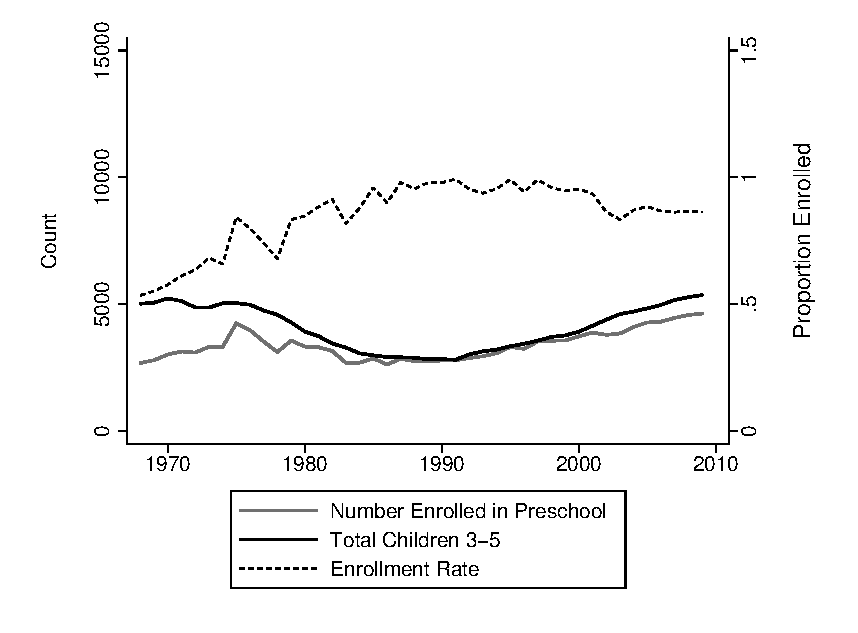
\includegraphics[width=\textwidth]{../../output/image/enrollment_vs_totalChildren_Reggio.eps}
%\end{subfigure}%
%~
%\begin{subfigure}[b]{0.55\textwidth}
%	\caption{Padova}\label{fig:enrollmentRatePadova}
%	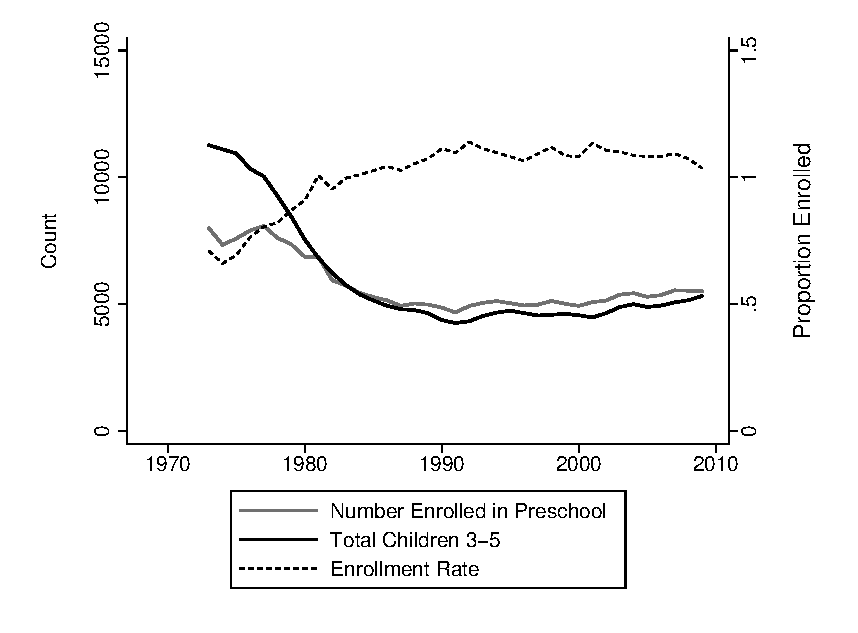
\includegraphics[width=\textwidth]{../../output/image/enrollment_vs_totalChildren_Padova.eps}
%\end{subfigure}%
%\end{center}
%\raggedright \footnotesize Note: These graphs show the trend in enrollment rates in Reggio Emilia and Padova over time. The series measuring preschool enrollment is not restricted to the 3-5 age group, and thus, is allowed to be greater than the series for total children 3-5. The enrollment proportion is occasionally greater than 1 in Padova due to this reason. See Appendix~\ref{app:characteristics-cities} for information on the sources used to construct these graphs.
%\end{figure}
%
%This information provides evidence of the extent to which alternative preschools were available and utilized. Comparing a individuals who attended one preschool program to those who attended another one can result in few outcomes, especially if the alternative preschools offer quality education. In fact, when we compare adults who attended some types of preschool in Padova with adults who did not attend any preschool in Padova, the estimation results show that the preschool attendance in Padova has significantly positive effects on IQ, university graduation, obesity, and voting behaviors for the age-30 cohort (See Appendix \ref{subsection:padova-estimation} for more specific results). This suggests that Padova had quality preschool education system from the 1970s. 

\clearpage

\bibliography{heckman}
\bibliographystyle{chicago}


\end{document}
